%$Header: /home/dashley/cvsrep/e3ft_gpl01/e3ft_gpl01/webprojs/pamc/gen_a/docs/manual/man_a/c_tbg0/c_tbg0.tex,v 1.35 2009/11/01 02:42:55 dashley Exp $

\chapter{Technical Background and Decisions}

\label{ctbg0}

\beginchapterquote{``The purpose of computing is insight, not numbers.''}
                  {Richard W. Hamming, 1962}

%%%%%%%%%%%%%%%%%%%%%%%%%%%%%%%%%%%%%%%%%%%%%%%%%%%%%%%%%%%%%%%%%%%%%%%%%%%%%%%
%%%%%%%%%%%%%%%%%%%%%%%%%%%%%%%%%%%%%%%%%%%%%%%%%%%%%%%%%%%%%%%%%%%%%%%%%%%%%%%
%%%%%%%%%%%%%%%%%%%%%%%%%%%%%%%%%%%%%%%%%%%%%%%%%%%%%%%%%%%%%%%%%%%%%%%%%%%%%%%
\section{Introduction}
%Section tag:  INT0
\label{ctbg0:sint0}

This chapter provides technical background and describes key 
\emph{\productbasename{}}
technical
and design decisions.


%%%%%%%%%%%%%%%%%%%%%%%%%%%%%%%%%%%%%%%%%%%%%%%%%%%%%%%%%%%%%%%%%%%%%%%%%%%%%%%
%%%%%%%%%%%%%%%%%%%%%%%%%%%%%%%%%%%%%%%%%%%%%%%%%%%%%%%%%%%%%%%%%%%%%%%%%%%%%%%
%%%%%%%%%%%%%%%%%%%%%%%%%%%%%%%%%%%%%%%%%%%%%%%%%%%%%%%%%%%%%%%%%%%%%%%%%%%%%%%
\section{Technical Background}
%Section tag:  tbg0
\label{ctbg0:stbg0}


%%%%%%%%%%%%%%%%%%%%%%%%%%%%%%%%%%%%%%%%%%%%%%%%%%%%%%%%%%%%%%%%%%%%%%%%%%%%%%%
%%%%%%%%%%%%%%%%%%%%%%%%%%%%%%%%%%%%%%%%%%%%%%%%%%%%%%%%%%%%%%%%%%%%%%%%%%%%%%%
%%%%%%%%%%%%%%%%%%%%%%%%%%%%%%%%%%%%%%%%%%%%%%%%%%%%%%%%%%%%%%%%%%%%%%%%%%%%%%%
\subsection{The SHA1 Secure Hash Algorithm}
%Subsection tag:  sha0
\label{ctbg0:stbg0:ssha0}

The SHA1 secure hash algorithm is described by 
\index{RFC 3174}RFC 3174
(available many places on the Internet).  The algorithm maps from
a block of data of any practical length to a 160-bit hash.  The important features of
the algorithm are described in the executive summary of RFC 3174:

\begin{quote}
\emph{This document specifies a Secure Hash Algorithm, SHA-1, for computing
a condensed representation of a message or a data file.  When a
message of any length $<$ $2^{64}$ bits is input, the SHA-1 produces a
160-bit output called a message digest.  The message digest can then,
for example, be input to a signature algorithm which generates or
verifies the signature for the message.  Signing the message digest
rather than the message often improves the efficiency of the process
because the message digest is usually much smaller in size than the
message.  The same hash algorithm must be used by the verifier of a
digital signature as was used by the creator of the digital
signature.  Any change to the message in transit will, with very high
probability, result in a different message digest, and the signature
will fail to verify.}

\emph{The SHA-1 is called secure because it is computationally infeasible
to find a message which corresponds to a given message digest, or to
find two different messages which produce the same message digest.
Any change to a message in transit will, with very high probability,
result in a different message digest, and the signature will fail to
verify.}
\end{quote}

The SHA1 algorithm is used for several purposes within
\emph{\productbasename{}-\productversion{}}:

\begin{itemize}
\item Rather than storing user passwords plain, 
      the standard hash\index{standard hash function} (\S{}\ref{ctbg0:sddc0:sshf0}) of each
      user password is stored.  The standard hash is
      based on the SHA1 algorithm.  (A hash
      is used because of the non-reversibility---it isn't
      possible to go backwards from the hash to the password.)
\item Session identifiers (SIDs, \S{}\ref{ctbg0:sdty0:ssid0})
      are based on the SHA1 function.  (It isn't possible for
      an attacker to guess the exact form of a SID because of
      the construction of the hash.)
\item The SHA1 hash is calculated for files stored in the
      file repository, and this information is retained in the
      database record corresponding to the file.  This serves
      three purposes:
      
      \begin{itemize}
      \item It allows the file to be periodically checked for corruption
            (due to hard disk failure or software defects).
      \item It allows users who upload a file to be sure that it
            was uploaded without corruption.
      \item It allows users who download a file to be sure that
            it was downloaded without corruption.
      \end{itemize} 
\end{itemize}


%%%%%%%%%%%%%%%%%%%%%%%%%%%%%%%%%%%%%%%%%%%%%%%%%%%%%%%%%%%%%%%%%%%%%%%%%%%%%%%
%%%%%%%%%%%%%%%%%%%%%%%%%%%%%%%%%%%%%%%%%%%%%%%%%%%%%%%%%%%%%%%%%%%%%%%%%%%%%%%
%%%%%%%%%%%%%%%%%%%%%%%%%%%%%%%%%%%%%%%%%%%%%%%%%%%%%%%%%%%%%%%%%%%%%%%%%%%%%%%
\section{Data Types}
%Section tag:  dty0
\label{ctbg0:sdty0}

\emph{PHP} has several native data types, including
integers and strings.  \emph{PHP} handles
strings well, and so ``custom'' data types are
in most cases most conveniently represented as strings (although
sometimes arrays of integers, arrays of strings, or some combination
is most convenient).  This section for the
most part describes the ``custom'' data types 
used in the \emph{\productbasename{}-\productversion{}} software.


%%%%%%%%%%%%%%%%%%%%%%%%%%%%%%%%%%%%%%%%%%%%%%%%%%%%%%%%%%%%%%%%%%%%%%%%%%%%%%%
%%%%%%%%%%%%%%%%%%%%%%%%%%%%%%%%%%%%%%%%%%%%%%%%%%%%%%%%%%%%%%%%%%%%%%%%%%%%%%%
%%%%%%%%%%%%%%%%%%%%%%%%%%%%%%%%%%%%%%%%%%%%%%%%%%%%%%%%%%%%%%%%%%%%%%%%%%%%%%%
\subsection{Hash Key}
%Subsection tag:  thk0
\label{ctbg0:sdty0:sthk0}

\index{hash key}Some of the 
security of \emph{\productbasename{}-\productversion{}} is based
on an attacker's inability to determine in advance what hash value will
be paired with data by the \emph{\productbasename{}-\productversion{}}.
Because the source code of \emph{\productbasename{}-\productversion{}} is
public, it is necessary to have an element of hash calculation that is not
known to an attacker.

The unknown random element is called the 
\index{hash key}\emph{hash key}.  The hash key is a string consisting
(quite arbitrarily) of printable characters.

A reasonable guideline for the length $n$ of the hash key is that it
should have at least as many possible values as the hash output
that it influences.  Assuming that lower- and upper-case letters
and digits are used (62 possibilities):

\begin{eqnarray}
\label{eq:ctbg0:sdty0:sthk0:01} 62^n & \geq & 2^{160} \\
\label{eq:ctbg0:sdty0:sthk0:02} n & \geq & \frac{160 \log 2}{\log 62} \approx 27
\end{eqnarray}

A hash key of 100 characters each chosen from letters and digits
should thus be more than adequate to prevent attacks.

The hash key is most readily generated by the 
\index{hashkeygen@\emph{hashkeygen}}\emph{hashkeygen} program,
described in \S{}\ref{csco0:ssph0:shkg0} (p. \pageref{csco0:ssph0:shkg0})
and in \S{}\ref{cist0:scsh0} (p. \pageref{cist0:scsh0}).
The \emph{hashkeygen} program generates a hash key substantially
longer than the threshold suggested
by Eq. \ref{eq:ctbg0:sdty0:sthk0:02} (see 
Fig. \ref{fig:cist0:scsh0:01}, p. \pageref{fig:cist0:scsh0:01}).


%%%%%%%%%%%%%%%%%%%%%%%%%%%%%%%%%%%%%%%%%%%%%%%%%%%%%%%%%%%%%%%%%%%%%%%%%%%%%%%
%%%%%%%%%%%%%%%%%%%%%%%%%%%%%%%%%%%%%%%%%%%%%%%%%%%%%%%%%%%%%%%%%%%%%%%%%%%%%%%
%%%%%%%%%%%%%%%%%%%%%%%%%%%%%%%%%%%%%%%%%%%%%%%%%%%%%%%%%%%%%%%%%%%%%%%%%%%%%%%
\subsection{AUTIME (Augmented Unix Timestamp)}
%Subsection tag:  ati0
\label{ctbg0:sdty0:sati0}

\index{AUTIME}%
An \emph{augmented Unix timestamp} is a decimal representation of the number of
seconds since Jan 1, 1900 GMT, and includes a fractional part.  Note that for times
after Jan 1, 1970 GMT, the AUTIME can be formed in a straightforward way from
the standard Unix time by adding a constant.

\begin{figure}
\centering
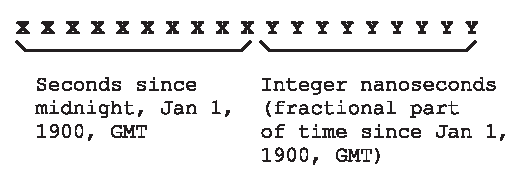
\includegraphics[width=4.6in]{c_tbg0/autimeformat01.eps}
\caption{Format of AUTIME}
\label{fig:ctbg0:sdty0:sati0:00}
\end{figure}

Figure \ref{fig:ctbg0:sdty0:sati0:00} illustrates the format of
an AUTIME\@.  An AUTIME is a string consisting
of exactly 19 characters, with the following
components.

\begin{itemize}
\item \textbf{Integer seconds since midnight, January 1, 1900 GMT (10 characters):}
      These 10 characters are a decimal integer, zero-padded on the left as
      necessary, that represent the integer seconds since midnight, January 1,
      1900 GMT.
\item \textbf{Nanoseconds associated with the integer seconds (9 characters):}
      These 9 characters are an integer, zero-padded on the left as
      necessary, that represent the nanoseconds associated with the
      integer seconds since the midnight, January 1, 1900 GMT.  
\end{itemize}

\index{leap second}Leap seconds are handled by ignoring them.
In essence, a ``virtual timespace'' is created where every day is exactly
86,400 seconds long and leap seconds don't exist.  This strategy is
very similar to the notion of Unix time except that leap seconds are
avoided.  The strategy has these components:

\begin{itemize}
\item Past and future times may be translated into an AUTIME that is
      either ambiguous or non-existent in the presence of leap seconds (this could
      occur only for a time within one second of midnight).
\item When an AUTIME is obtained from the PHP library functions included with
      \emph{\productbasename{}-\productversion{}}, a time within one
      second of midnight Unix time\footnote{Midnight UTC.} won't be supplied (instead, the
      library function will \index{sleep}sleep or spin-lock 
      until the two-second window of vulnerability has passed).
      This behavior is designed to avoid supplying ambiguous times or
      reverse-ordered times.
\item Time differences calculated using two AUTIMEs may differ from the
      actual time difference by up to the number of leap seconds that
      have occurred between the two AUTIMEs.\footnote{In practice, this
      is a very small error, bounded at several seconds per year.}      
\end{itemize}

Note that AUTIMEs as described have the property that the lexical
string sort order corresponds to the time sort order.

The calendaring range of an AUTIME spans:

\begin{itemize}
\item Midnight on January 1, 1900, GMT, \emph{through}
\item One nanosecond before midnight on January 1, 2200, UTC.
\end{itemize}

\noindent{}The calendaring range was chosen to allow the representation of
past events (such as birthdays), but also to allow dates substantially
in the future. 

In addition, the following values are reserved.
In each of the descriptions below, each ``X'' character
signifies a ``don't care'' (the ``X'' characters
are ignored in comparisons).

\begin{itemize}
\item \emph{9999999996XXXXXXXXX} is reserved to
      indicate an underflow result, i.e. a time
      before January 1, 1900, GMT.
\item \emph{9999999997XXXXXXXXX} is reserved to
      indicate an overflow result, i.e. a time
      after one nanosecond before 
      January 1, 1200, UTC.
\item \emph{9999999998XXXXXXXXX} is reserved to
      indicate an indeterminate time, i.e. the
      time can't be reliably determined.
\item \emph{9999999999XXXXXXXXX} is reserved to
      indicate an otherwise unspecified error.
\item Values corresponding to a time of at least
      midnight, January 1, 2200, UTC but less than 
      \emph{9999999996XXXXXXXXX} are treated
      as \emph{9999999999XXXXXXXXX}.  These
      values should never occur in practice as the
      date arithmetic functions should not allow these
      values to be calculated as output.
\end{itemize}

Note that the AUTIME format can be used for values that:

\begin{itemize}
\item Are used as part of generating a unique or random data value
      (see, for example, \S{}\ref{ctbg0:sdty0:ssgu0}).
\item Are used to determine elapsed time.
\end{itemize}


%%%%%%%%%%%%%%%%%%%%%%%%%%%%%%%%%%%%%%%%%%%%%%%%%%%%%%%%%%%%%%%%%%%%%%%%%%%%%%%
%%%%%%%%%%%%%%%%%%%%%%%%%%%%%%%%%%%%%%%%%%%%%%%%%%%%%%%%%%%%%%%%%%%%%%%%%%%%%%%
%%%%%%%%%%%%%%%%%%%%%%%%%%%%%%%%%%%%%%%%%%%%%%%%%%%%%%%%%%%%%%%%%%%%%%%%%%%%%%%
\subsection{AUTIMEIP (Augmented Unix Timestamp Integer Pair)}
%Subsection tag:  ati2
\label{ctbg0:sdty0:sati2}

\index{AUTIMEIP}The string representation of an AUTIME is most convenient for
string manipulation in \emph{PHP}.  However, for manipulation 
in \emph{MySQL} and in CGI-BIN programs it may be more efficient to
represent the AUTIME as a pair of integers; one for the whole seconds
and one for the fractional nanoseconds.  This represesentation as a pair
of integers is the AUTIMEIP data type.

As of January 1, 2200, there will have been approximately
9,467,280,000 seconds since January 1, 1900.  The whole number
of seconds requires 34 bits to represent, and so this is compatible
with the \emph{MySQL} \emph{bigint} data type (but incompatible with
native \emph{PHP} integers with \emph{PHP} version 4.X on 32-bit
platforms).

The number of fractional nanoseconds $n$ always meets the
constraint $0 \leq n \leq 999,999,999$ and thus requires
30 bits to represent.  This integer is compatible with
the \emph{MySQL} \emph{int} data type and with \emph{PHP}
integers.

An AUTIMEIP may be represented in the following ways:

\begin{itemize}
\item A \emph{bigint}/\emph{int} pair in \emph{MySQL}.
\item A 64-bit/32-bit integer pair in a compiled C program.
\item A string/integer pair in \emph{PHP}, where the string
      is manipulated using \emph{bcmath} and the integer
      is manipulated as provided for in the language.
\end{itemize}

The exception values as described in \S{}\ref{ctbg0:sdty0:sati0}
also apply to AUTIMEIP values.


%%%%%%%%%%%%%%%%%%%%%%%%%%%%%%%%%%%%%%%%%%%%%%%%%%%%%%%%%%%%%%%%%%%%%%%%%%%%%%%
%%%%%%%%%%%%%%%%%%%%%%%%%%%%%%%%%%%%%%%%%%%%%%%%%%%%%%%%%%%%%%%%%%%%%%%%%%%%%%%
%%%%%%%%%%%%%%%%%%%%%%%%%%%%%%%%%%%%%%%%%%%%%%%%%%%%%%%%%%%%%%%%%%%%%%%%%%%%%%%
\subsection{AUTIMEI (Augmented Unix Timestamp Integer)}
%Subsection tag:  ati3
\label{ctbg0:sdty0:sati3}

\index{AUTIMEI}On January 1, 2200 UTC, the number of nanoseconds since 
midnight January 1, 1900 GMT will be approximately 
$9.4673 \times 10^{18}$, requiring 
64 bits to represent.  The integer representation of
the number of nanoseconds since midnight January 1, 1900
is the AUTIMEI data type.

Note that the AUTIMEI data type cannot be represented in a 
\emph{MySQL} \emph{bigint}, as a \emph{MySQL} \emph{bigint}
can represent values only from $-2^{63}$ through $2^{63}-1$.

The AUTIMEI data type can often be represented in an integer
in the C programming langauge, as implementations often provide
for unsigned 64-bit integers.

The exception values as described in \S{}\ref{ctbg0:sdty0:sati0}
also apply to AUTIMEIP values.


%%%%%%%%%%%%%%%%%%%%%%%%%%%%%%%%%%%%%%%%%%%%%%%%%%%%%%%%%%%%%%%%%%%%%%%%%%%%%%%
%%%%%%%%%%%%%%%%%%%%%%%%%%%%%%%%%%%%%%%%%%%%%%%%%%%%%%%%%%%%%%%%%%%%%%%%%%%%%%%
%%%%%%%%%%%%%%%%%%%%%%%%%%%%%%%%%%%%%%%%%%%%%%%%%%%%%%%%%%%%%%%%%%%%%%%%%%%%%%%
\subsection{AUTIMELP (Augmented Unix Timestamp, Low Precision)}
%Subsection tag:  ati1
\label{ctbg0:sdty0:sati1}

\index{AUTIMELP}The augmented Unix time is also manipulated in the
software without the fractional part.  Such values are used where
a precision of one second is adequate.

An AUTIMELP is a string of exactly 10 characters.
The ranges and exception values specified in 
\S{}\ref{ctbg0:sdty0:sati1} apply.


%%%%%%%%%%%%%%%%%%%%%%%%%%%%%%%%%%%%%%%%%%%%%%%%%%%%%%%%%%%%%%%%%%%%%%%%%%%%%%%
%%%%%%%%%%%%%%%%%%%%%%%%%%%%%%%%%%%%%%%%%%%%%%%%%%%%%%%%%%%%%%%%%%%%%%%%%%%%%%%
%%%%%%%%%%%%%%%%%%%%%%%%%%%%%%%%%%%%%%%%%%%%%%%%%%%%%%%%%%%%%%%%%%%%%%%%%%%%%%%
\subsection{UBDT (Unbound Date)}
%Subsection tag:  ubd0
\label{ctbg0:sdty0:subd0}

It is occasionally desirable to specify a date in a context where a narrow
or unique mark or range in time isn't important or can't be determined.
An example would be
a birthday---a birthday alone gives no indication of the global time zone
where the person was born (and hence the range of times
potentially represented by the date
would be interpreted differently at different global locations).

These vague dates are called \index{unbound date}\emph{unbound dates}. 

Unbound dates are in general unsuitable for most applications within 
\emph{\productbasename{}-\productversion{}}\@.  Even software release dates
are best maintained as AUTIMEs---for example, a software release on a
certain date in the U.S.
might be best thought of as occurring on the following day in Europe.

Unbound dates are always represented within the
\emph{\productbasename{}-\productversion{}} software in the form
\emph{YYYYMMDD}, and may range from 19000101 to 
21991231, inclusive.

The value \emph{00000000} is used to represent an underflow (date before January
1, 1900), the value \emph{99999999} is used to represent an overflow (date
after December 31, 2199), and the value \emph{--------} is used to represent
any other type of error.

The \emph{PHP} library files in \emph{\productbasename{}-\productversion{}}
include functions to perform calculations with unbound dates.


%%%%%%%%%%%%%%%%%%%%%%%%%%%%%%%%%%%%%%%%%%%%%%%%%%%%%%%%%%%%%%%%%%%%%%%%%%%%%%%
%%%%%%%%%%%%%%%%%%%%%%%%%%%%%%%%%%%%%%%%%%%%%%%%%%%%%%%%%%%%%%%%%%%%%%%%%%%%%%%
%%%%%%%%%%%%%%%%%%%%%%%%%%%%%%%%%%%%%%%%%%%%%%%%%%%%%%%%%%%%%%%%%%%%%%%%%%%%%%%
\subsection{SGUID (Server Globally-Unique Identifier)}
%Subsection tag:  sgu0
\label{ctbg0:sdty0:ssgu0}

It is necessary or helpful in some contexts to have a way to create an
identifier that is guaranteed to occur no more often than once in the lifetime
of the server.  \emph{MySQL} can be used to create such identifiers, and there
are also methods based on file and IPC semantics that can be used.

The method used in the software is a \index{spin lock}spin lock on a precision
timestamp; and the timestamp is concatenated with the PID.  The method works
because:

\begin{itemize}
\item A single process (by virtue of the spin lock) can't generate the same
      precision timestamp twice.
\item No two processes can have the same PID at the same time.
\end{itemize}

\begin{figure}
\centering
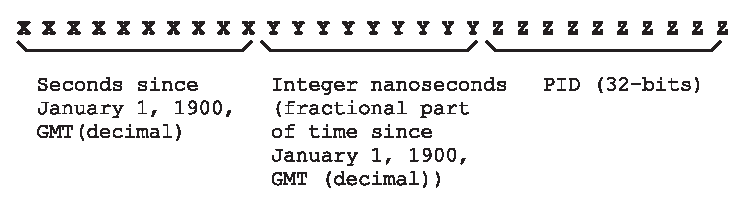
\includegraphics[width=4.6in]{c_tbg0/sguidformat01.eps}
\caption{Format of SGUID}
\label{fig:ctbg0:sdty0:ssgu0:00}
\end{figure}

Figure \ref{fig:ctbg0:sdty0:ssgu0:00} illustrates the format of
an SGUID.  An SGUID consists of 29 characters, with the following
components.

\begin{itemize}
\item \textbf{Integer seconds since the January 1, 1900 GMT (10 characters):}
      These 10 characters are an integer, zero-padded on the left as
      necessary, that represent the integer seconds since January 1, 1900
      GMT.\footnote{Note that 10 digits comfortably solves the Unix
      2037 A.D. issue, as this will guarantee SGUIDs 
      beyond 2200 A.D.}
\item \textbf{Nanoseconds associated with the integer seconds (9 characters):}
      These 9 characters are an integer, zero-padded on the left as
      necessary, that represent the nanoseconds associated with the
      integer seconds since January 1, 1900,
      GMT.\footnote{As of this writing, Linux provides time to a resolution
      of microseconds.  It is anticipated that a resolution of nanoseconds will
      accommodate any hardware speed advances in the foreseeable future, as typical
      hardware gate propagation delays are on the order of several nanoseconds.}  
\item \textbf{PID (10 characters):}
      These 10 characters are an integer, zero-padded on the left as
      necessary, that represent Unix PID expressed 
      as a decimal number.\footnote{As of this writing, PIDs are 16 bits only.
      However, it seems inevitable that PIDs will be expanded to 24 or 32 bits in the 
      future.}  
\end{itemize}

Note that SGUIDs as described have a very important property in addition to
guaranteed uniqueness---the lexical
string sort order corresponds to the time sort order.

Two sample applications of SGUIDs are:

\begin{itemize}
\item The basis for a session identifier (guaranteed unique).
\item A field in a database record to detect browser editing collisions---when a record
      is modified and a new SGUID is assigned to the record, it is \emph{guaranteed}
      not to be the same as the previous SGUID, and thus detection of the editing collision
      is guaranteed.
\end{itemize}


%%%%%%%%%%%%%%%%%%%%%%%%%%%%%%%%%%%%%%%%%%%%%%%%%%%%%%%%%%%%%%%%%%%%%%%%%%%%%%%
%%%%%%%%%%%%%%%%%%%%%%%%%%%%%%%%%%%%%%%%%%%%%%%%%%%%%%%%%%%%%%%%%%%%%%%%%%%%%%%
%%%%%%%%%%%%%%%%%%%%%%%%%%%%%%%%%%%%%%%%%%%%%%%%%%%%%%%%%%%%%%%%%%%%%%%%%%%%%%%
\subsection{SID (Session Identifier)}
%Subsection tag:  sid0
\label{ctbg0:sdty0:ssid0}

A \index{session identifier}session identifier (\index{SID}SID) is a
string consisting of exactly 69 characters used to uniquely
identify a session (Figure \ref{fig:ctbg0:sdty0:ssid0:00}).

\begin{figure}
\centering
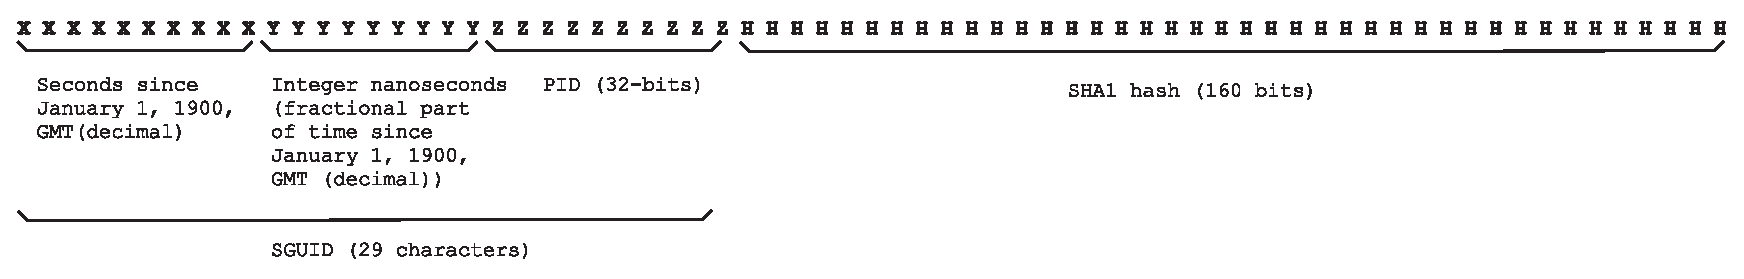
\includegraphics[width=4.6in]{c_tbg0/sidformat01.eps}
\caption{Format of SID}
\label{fig:ctbg0:sdty0:ssid0:00}
\end{figure}

The first part of the SID is a SGUID 
(\S{}\ref{ctbg0:sdty0:ssgu0}).  The second part of a SID is
the system hash function of the SGUID.  The SGUID portion is guaranteed to
be unique (this is a defining property of an SGUID),
and so each SID is unique within the first 29 characters.
The SHA1 hash appended to the SGUID is designed to eliminate an attacker's
ability to construct a valid SID.  It may be possible to guess an SGUID based
on server characteristics; but it should not be possible to guess the corresponding
hash (this is a defining property of the system hash function).

At the time a user logs in (either as a user or a guest), the SID is created
and provided to the browser as a cookie.

The session state changes that occur as \emph{\productbasename{}-\productversion{}}
is used are all stored on the server side.  The advantages of this approach
are:

\begin{itemize}
\item Only one cookie of a very short length is stored in the client's browser.
      This approach meets the RFC 2109 constraints and is also suitable
      for mobile devices.
\item An attacker's ability to gather information about the internal workings
      of \emph{\productbasename{}-\productversion{}} by
      observing cookie reassignments is severely limited
      (nothing except the SID is exposed, and exposed only once per session).
\item An attacker's ability to tamper with cookies is eliminated (only one
      cookie is provided, and it is tamper-proof).       
\end{itemize}


%%%%%%%%%%%%%%%%%%%%%%%%%%%%%%%%%%%%%%%%%%%%%%%%%%%%%%%%%%%%%%%%%%%%%%%%%%%%%%%
%%%%%%%%%%%%%%%%%%%%%%%%%%%%%%%%%%%%%%%%%%%%%%%%%%%%%%%%%%%%%%%%%%%%%%%%%%%%%%%
%%%%%%%%%%%%%%%%%%%%%%%%%%%%%%%%%%%%%%%%%%%%%%%%%%%%%%%%%%%%%%%%%%%%%%%%%%%%%%%
\section{Database Design Decisions and Discussion}
%Section tag:  ddd0
\label{ctbg0:sddd0}


%%%%%%%%%%%%%%%%%%%%%%%%%%%%%%%%%%%%%%%%%%%%%%%%%%%%%%%%%%%%%%%%%%%%%%%%%%%%%%%
%%%%%%%%%%%%%%%%%%%%%%%%%%%%%%%%%%%%%%%%%%%%%%%%%%%%%%%%%%%%%%%%%%%%%%%%%%%%%%%
%%%%%%%%%%%%%%%%%%%%%%%%%%%%%%%%%%%%%%%%%%%%%%%%%%%%%%%%%%%%%%%%%%%%%%%%%%%%%%%
\subsection{Global Scope Naming Conventions}
%Subsection tag:  gsn0
\label{ctbg0:sddd0:sgsn0}

In certain of the database tables and in certain other
contexts, a global naming convention is used rather than
further indexing information by application and page.  (For
example, the \emph{upns} and \emph{stns} tables in 
\S{}\ref{ctbg0:sddd0:scfn0}, Figure
\ref{fig:ctbg0:sddd0:scfn0:spga0:00}, p. 
\pageref{fig:ctbg0:sddd0:scfn0:spga0:00}.)

The conventions are quite loose, and simply consist of assigning names
that suggest, in order, the application, then the page, then the 
variable within the page.
If this convention is followed, applications and pages can easily
query for all the database records that affect them by using the
SQL \emph{like} clause.\footnote{It was verified that \emph{MySQL} will
perform such a query nearly instantly even with a million records, so long
as the column involved in the query is indexed and so long as the wildcard
part of the name is at the end.}

For example, a \emph{MySQL} query of the form\\\\
\texttt{SELECT * FROM tablename\\WHERE columnname LIKE 'APP\_\%' ORDER BY columnname;}\\\\
will very efficiently extract all records whose value in a column
begins with ``APP\_'', so long as the column is indexed.

Using these naming conventions, it is also possible to simulate arrays.  For
example, a variable named\\\\
\texttt{APP\_EMPCOST\_PG\_RECORDDISPLAY\_EMP\_HRS\_000029\_000042}\\\\
might be used to represent row 29 and column 42 of the underlying variable.


%%%%%%%%%%%%%%%%%%%%%%%%%%%%%%%%%%%%%%%%%%%%%%%%%%%%%%%%%%%%%%%%%%%%%%%%%%%%%%%
%%%%%%%%%%%%%%%%%%%%%%%%%%%%%%%%%%%%%%%%%%%%%%%%%%%%%%%%%%%%%%%%%%%%%%%%%%%%%%%
%%%%%%%%%%%%%%%%%%%%%%%%%%%%%%%%%%%%%%%%%%%%%%%%%%%%%%%%%%%%%%%%%%%%%%%%%%%%%%%
\subsection{\emph{MySQL} Database Locking}
%Subsection tag:  mdl0
\label{ctbg0:sddd0:smdl0}

The design of \emph{\productbasename{}-\productversion{}} includes
many tables and complex relations.  In order to ensure database
consistency, it is necessary to ensure atomicity of operations.

The approach taken to serialize database access is:

\begin{itemize}
\item Serialization is accomplished via the SQL \emph{LOCK TABLES}
      and \emph{UNLOCK TABLES} statements.

      \begin{itemize}
      \item At the start of the critical section, \emph{all} tables existing
            in the database are locked via a single \emph{LOCK TABLES}
            statement.\footnote{It was determined via newsgroup posts
            that the practical limit on the number of tables that can 
            be locked in a single SQL statement is much higher---probably
            thousands of tables---than will be encountered in practice in
            this product.  As a fallback position if locking all tables
            proves impossible, the \emph{GET\_LOCK()} 
            function and its companion function can be used.  \emph{GET\_LOCK()}
            isn't the first choice because the name is server-global rather
            than database global, and malicious code (in another database
            application) could cause denial of service.  Additionally, it has
            been verified that this method handles all the important scenarios
            such as ordinary contention, dying processes, a process that 
            terminates without releasing the lock, etc.}
      \item At the end of the critical section, a single \emph{UNLOCK TABLES}
            statement is executed.
      \end{itemize}
\item Maintenance scripts that run hot will be written to lock and unlock so that
      if there is collision with a web page, the web page will be delayed for only
      a small amount of time.
\item A recursive locking protocol is employed in the software to simplify the case
      of a critical section occurring within a critical section.  (This ensures
      in an orderly way
      that large-scope critical sections are not compromised by small-scope critical
      sections.)
\end{itemize}


%%%%%%%%%%%%%%%%%%%%%%%%%%%%%%%%%%%%%%%%%%%%%%%%%%%%%%%%%%%%%%%%%%%%%%%%%%%%%%%
%%%%%%%%%%%%%%%%%%%%%%%%%%%%%%%%%%%%%%%%%%%%%%%%%%%%%%%%%%%%%%%%%%%%%%%%%%%%%%%
%%%%%%%%%%%%%%%%%%%%%%%%%%%%%%%%%%%%%%%%%%%%%%%%%%%%%%%%%%%%%%%%%%%%%%%%%%%%%%%
\subsection{File Repository Organization}
%Subsection tag:  fro0
\label{ctbg0:sddd0:sfro0}

The \emph{\productbasename{}} software needs to maintain user-uploaded
files in conjunction with a 
database.  All such files are aggregated into one structure
called the \emph{file repository}.\index{file repository}

In the type of file repository described here, each file in the repository
has a corresponding database record containing a unique integer index.  These indices
are assigned automatically by \emph{MySQL} and are assigned sequentially
as files are added (i.e. ``1'', ``2'', ``3'', etc.).

Although
\emph{MySQL} has the capability to store files directly as part of
the database, the files are stored as distinct files directly
under the operating system for the following
reasons:

\begin{itemize}
\item The upper limit for the size of the individual and collective
      files stored directly in 
      \emph{MySQL} is not known or trusted.  (The behavior of 
      the *nix filesystem, on the other hand, is well-understood
      and trusted.)
\item The ability to split the file repository across multiple
      volumes (for disk capacity reasons) via symlinks must
      be preserved.
\item In the event of \emph{MySQL} database corruption, the files must still
      be easily recoverable.  This constraint would not be met if the
      files were stored directly in \emph{MySQL}.
\item If incremental backups are used, it is known that \emph{MySQL} tends
      to cause an entire table of files to be backed up (this can be tens
      or hundreds of megabytes or more), whereas an approach relying on discrete
      files will cause only the new or modified files to be incrementally
      backed up.
\end{itemize}

The following constraints and design goals for the file repository exist:

\begin{itemize}
\item The differential growth of disk consumption due to overhead (such as
      directory creation) as files are added
      should not be excessive under the assumption that indices grow linearly. 
\item It is known that *nix systems begin to experience performance issues
      when directories contain more than about 200 files or subdirectories (due to
      the linear search).  Any solution should not place more than about 200 files
      or subdirectories in a directory.
\item The solution should facilitate symlinking to split the file
      repository across multiple volumes.
\item The solution must accommodate logical indices as large as $2^{64}-1$.\footnote{This design
      goal applies because \emph{MySQL} allows 64-bit integers to be used as the primary
      key for database tables.}
\item The solution must allow files to be aged out or deleted
      randomly with respect to the integer indices (to comply with records retention
      policies, because they are removed from the repository, or for other reasons).
\end{itemize}

In order to accommodate the constraints, files are stored in a directory structure
based on prime moduli of the database integer index $n$.  
The lowest level of the directory structure contains a single
file per directory, with the lowest-level directory named being the 
decimal representation of the
integer index $n$.

The definining equations for the directory path components are supplied below.

\begin{eqnarray}
\label{eq:ctbg0:sddd0:sfro0:00}   d    & = & 160                               \\
\label{eq:ctbg0:sddd0:sfro0:01} c_0    & = & \lfloor n / d \rfloor \bmod 7   \\
\label{eq:ctbg0:sddd0:sfro0:02} c_1    & = & \lfloor n / d \rfloor \bmod 11  \\ 
\label{eq:ctbg0:sddd0:sfro0:03} c_2    & = & \lfloor n / d \rfloor \bmod 13  \\
\label{eq:ctbg0:sddd0:sfro0:04} c_3    & = & \lfloor n / d \rfloor \bmod 89  \\
\label{eq:ctbg0:sddd0:sfro0:05} c_4    & = & \lfloor n / d \rfloor \bmod 97  \\
\label{eq:ctbg0:sddd0:sfro0:06} c_5    & = & \lfloor n / d \rfloor \bmod 101 \\
\label{eq:ctbg0:sddd0:sfro0:07} c_6    & = & \lfloor n / d \rfloor \bmod 103 \\
\label{eq:ctbg0:sddd0:sfro0:08} c_7    & = & \lfloor n / d \rfloor \bmod 107 \\
\label{eq:ctbg0:sddd0:sfro0:09} c_8    & = & \lfloor n / d \rfloor \bmod 109 \\
\label{eq:ctbg0:sddd0:sfro0:10} c_9    & = & \lfloor n / d \rfloor \bmod 113 
\end{eqnarray}

With reference to (\ref{eq:ctbg0:sddd0:sfro0:01})
through (\ref{eq:ctbg0:sddd0:sfro0:10}), the relative path within a file repository
to the directory containing a file with database index $n$ is\\
``$c_0$/$c_1$/$c_2$/$c_3$/$c_4$/$c_5$/$c_6$/$c_7$/$c_8$/$c_9$/$n$''\@.
Each path component $c_i$ and $n$ is the traditional human-friendly variable-length
representation:
for example, ``3'', ``25'', ```111', or ``36237456726''.  

Note that the storage scheme proposed will handle indices 
as large as $2^{64}-1$, i.e.

\begin{equation}
\label{eq:ctbg0:sddd0:sfro0:20}
d \times c_0 \times c_1 \times c_2 \times c_3 \times c_4
\times c_5 \times c_6 \times c_7 \times c_8 \times c_9 > 2^{64} - 1 .
\end{equation}

Note also that the first three
components ($c_0$, $c_1$, and $c_2$) are small and chosen for 
convenient symlinking, whereas the last seven components ($c_3$ through $c_9$)
are chosen to increase the product rapidly while staying clear of the 
*nix performance limit of approximately 200 entries per directory.

Two properties of the storage scheme proposed by (\ref{eq:ctbg0:sddd0:sfro0:01})
through (\ref{eq:ctbg0:sddd0:sfro0:10}) may require further explanation.

\begin{itemize}
\item The differential cost of storing a file in the repository is
      approximately the file size (with operating system overhead)
      plus approximately 1.0625 directories.  This comes about because
      every file requires its own directory, and because
      every 160 files, 10 directories must be created.
\item If the index $n$ increases linearly, the number of files stored in
      each directory (especially at the top levels) will be approximately
      equal.  (The reason for this is the coprimality of the divisors
      used.  The necessary proof comes from number theory, and isn't 
      included here.)  This means that symlinking at the top levels will be
      effective in evenly dividing storage requirements.
\end{itemize}


%%%%%%%%%%%%%%%%%%%%%%%%%%%%%%%%%%%%%%%%%%%%%%%%%%%%%%%%%%%%%%%%%%%%%%%%%%%%%%%
%%%%%%%%%%%%%%%%%%%%%%%%%%%%%%%%%%%%%%%%%%%%%%%%%%%%%%%%%%%%%%%%%%%%%%%%%%%%%%%
%%%%%%%%%%%%%%%%%%%%%%%%%%%%%%%%%%%%%%%%%%%%%%%%%%%%%%%%%%%%%%%%%%%%%%%%%%%%%%%
\subsection{Database Design to Support Core Functionality}
%Subsection tag:  cfn0
\label{ctbg0:sddd0:scfn0}

The core functionality as described in Chapter \ref{ccfn0} consists of:

\begin{itemize}
\item Site navigation (\S{}\ref{ccfn0:ssng0}).
\item Authentication and login (\S{}\ref{ccfn0:salg0}).
\item Permission groups and attributes (\S{}\ref{ccfn0:sgra0}).
\item Notification (\S{}\ref{ccfn0:snot0}).
\item Action list (\S{}\ref{ccfn0:sacl0}).
\item Logging (\S{}\ref{ccfn0:slog0}).
\end{itemize}

Figure \ref{fig:ctbg0:sddd0:scfn0:spga0:00} provides an overview of the
tables involved in implementing the core functionality.  In the figure,
for efficiency, note that three of the most frequently
used read-only tables (\emph{applications}, \emph{pages},
and \emph{navlines}) are implemented as lookup tables in 
\emph{PHP} rather than
as \emph{MySQL} tables.\footnote{Presumably, the \emph{PHP}
interpreter parsing these tables is far more efficient than executing
an SQL query and processing the results.}

\begin{figure}
\centering
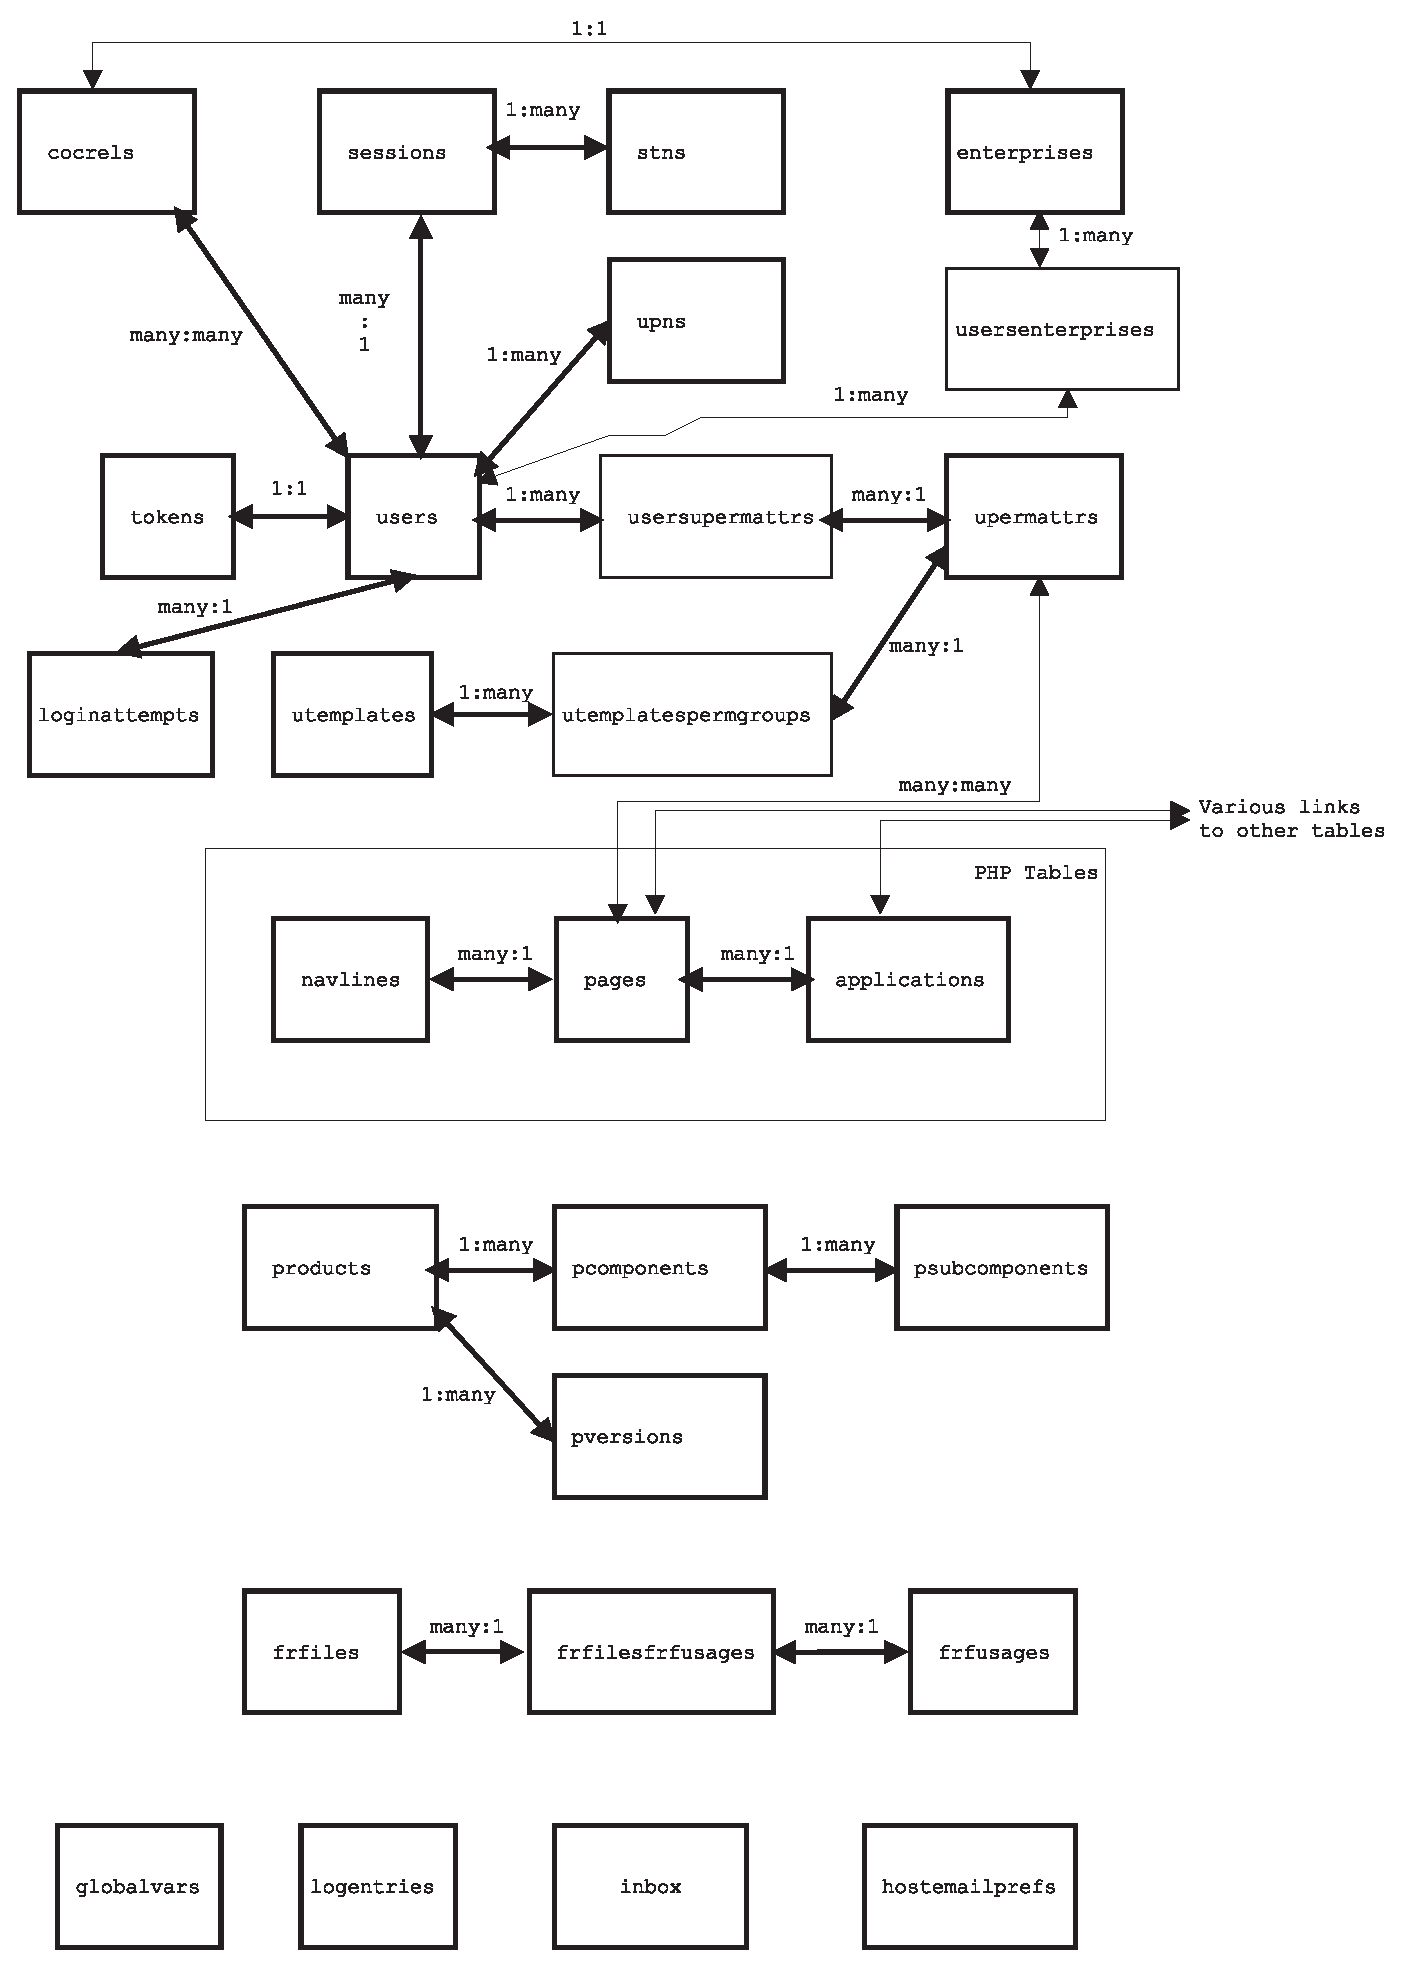
\includegraphics[width=4.6in]{c_tbg0/dbdesign01.eps}
\caption{User, Permission Group, Application, and Page Database Design}
\label{fig:ctbg0:sddd0:scfn0:spga0:00}
\end{figure}


%%%%%%%%%%%%%%%%%%%%%%%%%%%%%%%%%%%%%%%%%%%%%%%%%%%%%%%%%%%%%%%%%%%%%%%%%%%%%%%
%%%%%%%%%%%%%%%%%%%%%%%%%%%%%%%%%%%%%%%%%%%%%%%%%%%%%%%%%%%%%%%%%%%%%%%%%%%%%%%
%%%%%%%%%%%%%%%%%%%%%%%%%%%%%%%%%%%%%%%%%%%%%%%%%%%%%%%%%%%%%%%%%%%%%%%%%%%%%%%
\subsubsection{Users and Tokens}
%Subsubsection tag:  utk0
\label{ctbg0:sddd0:scfn0:sutk0}

The database design includes a table of users (the \emph{users} table
in Figure \ref{fig:ctbg0:sddd0:scfn0:spga0:00}).  Each user who can log
in to the system has one record in this table.  As mentioned
in \S{}????, each user always logs in using a userid that 
represents the user---there
are no userids used solely for administration.

The \emph{users} table 
(Figure \ref{fig:ctbg0:sddd0:scfn0:spga0:00}) is related 1:1 with the
\emph{tokens} table.
Each user is optionally assigned a cryptographic token to use in
authenticating.  Token assignment is on a per-user
basis, so that \emph{\productbasename{}-\productversion{}} will support:

\begin{itemize}
\item No users authenticating using cryptographic tokens.
\item Some users authenticating with cryptographic tokens, and some authenticating
      without cryptographic tokens.
\item All users authenticating with cryptographic tokens.
\end{itemize}


%%%%%%%%%%%%%%%%%%%%%%%%%%%%%%%%%%%%%%%%%%%%%%%%%%%%%%%%%%%%%%%%%%%%%%%%%%%%%%%
%%%%%%%%%%%%%%%%%%%%%%%%%%%%%%%%%%%%%%%%%%%%%%%%%%%%%%%%%%%%%%%%%%%%%%%%%%%%%%%
%%%%%%%%%%%%%%%%%%%%%%%%%%%%%%%%%%%%%%%%%%%%%%%%%%%%%%%%%%%%%%%%%%%%%%%%%%%%%%%
\subsubsection{User Permission Attributes}
%Subsubsection tag:  pga0
\label{ctbg0:sddd0:scfn0:spga0}

Figure \ref{fig:ctbg0:sddd0:scfn0:spga0:00} shows that the \emph{users} and 
\emph{upermattrs} tables are related by the \emph{userupermattrs} table, providing 
an $\infty{}:\infty{}$ mapping.

Each record in the \emph{userupermattrs} table also carries with it an
optional string.  Such as string is interpreted as a user-specific value of the
related record in the \emph{upermattrs} table.  As a 
contrived example, one user may have
a value of MAX\_LOGINS of 2, and another user may have a value of 5.

If the optional string in the \emph{userupermattrs} table is the empty string,
then the $\infty{}:\infty{}$ relation effectively specifies a named set
of users.  Such named sets are typically used to control user permissions
in a fine-grained way---a given group may contain the users who can add
products to the \emph{products} table, for example.


%%%%%%%%%%%%%%%%%%%%%%%%%%%%%%%%%%%%%%%%%%%%%%%%%%%%%%%%%%%%%%%%%%%%%%%%%%%%%%%
%%%%%%%%%%%%%%%%%%%%%%%%%%%%%%%%%%%%%%%%%%%%%%%%%%%%%%%%%%%%%%%%%%%%%%%%%%%%%%%
%%%%%%%%%%%%%%%%%%%%%%%%%%%%%%%%%%%%%%%%%%%%%%%%%%%%%%%%%%%%%%%%%%%%%%%%%%%%%%%
\subsubsection{User Persistent Named State}
%Subsubsection tag:  upn0
\label{ctbg0:sddd0:scfn0:supn0}

User permission attributes do not change as the result of ordinary usage of
the \emph{\productbasename{}-\productversion{}} system.  Although 
user permission attributes can be modified, this is an administrative action
and does not happen often.

For state bound to a user which may change often, the 
\emph{upns} table (Figure \ref{fig:ctbg0:sddd0:scfn0:spga0:00}) is
provided.  This state is very similar in spirit to what may be contained
in the \emph{Windows} registry.

Each record in the \emph{upns} table consists of a name and a value.

For each user, the names in the \emph{upns} table must be unique (no
duplicates are allowed).

A naming convention is used so that each entry in the \emph{upns} table
is bound to a specific application and page.  The \emph{upns} table is indexed
by name for fast retrieval.


%%%%%%%%%%%%%%%%%%%%%%%%%%%%%%%%%%%%%%%%%%%%%%%%%%%%%%%%%%%%%%%%%%%%%%%%%%%%%%%
%%%%%%%%%%%%%%%%%%%%%%%%%%%%%%%%%%%%%%%%%%%%%%%%%%%%%%%%%%%%%%%%%%%%%%%%%%%%%%%
%%%%%%%%%%%%%%%%%%%%%%%%%%%%%%%%%%%%%%%%%%%%%%%%%%%%%%%%%%%%%%%%%%%%%%%%%%%%%%%
\subsubsection{Sessions}
%Subsubsection tag:  ses0
\label{ctbg0:sddd0:scfn0:sses0}

A \emph{session} is the relationship between the server and a client during
a single login (whether as a named user or a guest).

Sessions are stored in the \emph{sessions} table 
(Figure \ref{fig:ctbg0:sddd0:scfn0:spga0:00}).  Each record in the 
\emph{sessions} table contains the session identifier, information about the
user, information about the time of the last actions associated with the
session, etc.


%%%%%%%%%%%%%%%%%%%%%%%%%%%%%%%%%%%%%%%%%%%%%%%%%%%%%%%%%%%%%%%%%%%%%%%%%%%%%%%
%%%%%%%%%%%%%%%%%%%%%%%%%%%%%%%%%%%%%%%%%%%%%%%%%%%%%%%%%%%%%%%%%%%%%%%%%%%%%%%
%%%%%%%%%%%%%%%%%%%%%%%%%%%%%%%%%%%%%%%%%%%%%%%%%%%%%%%%%%%%%%%%%%%%%%%%%%%%%%%
\subsubsection{Session Temporary Named State}
%Subsubsection tag:  stn0
\label{ctbg0:sddd0:scfn0:sstn0}

State that should be stored associated with a session rather than a user
(i.e. that should be deleted when a session ends) is stored in the
\emph{stns} table (Figure \ref{fig:ctbg0:sddd0:scfn0:spga0:00}).

Each entry in the \emph{stns} table consists of a name and a value.
Within each session, each name in the \emph{stns} table must be unique.

A naming convention is used so that each entry in the \emph{stns} table
is bound to a specific application and page.  The \emph{stns} table is indexed
by name for fast retrieval.


%%%%%%%%%%%%%%%%%%%%%%%%%%%%%%%%%%%%%%%%%%%%%%%%%%%%%%%%%%%%%%%%%%%%%%%%%%%%%%%
%%%%%%%%%%%%%%%%%%%%%%%%%%%%%%%%%%%%%%%%%%%%%%%%%%%%%%%%%%%%%%%%%%%%%%%%%%%%%%%
%%%%%%%%%%%%%%%%%%%%%%%%%%%%%%%%%%%%%%%%%%%%%%%%%%%%%%%%%%%%%%%%%%%%%%%%%%%%%%%
\subsubsection{Chain of Command}
%Subsubsection tag:  coc0
\label{ctbg0:sddd0:scfn0:scoc0}

In some contexts, \emph{\productbasename{}-\productversion{}} components
need to make decisions based on reporting relationships between
employees.  For example, some information about an employee should only
be viewable or editable by those above the employee in the chain of command.

The database contains an \emph{enterprises} table
(Figure \ref{fig:ctbg0:sddd0:scfn0:spga0:00}) and an
\emph{usersenterprises} table that provide a 
$\infty{}:\infty{}$ mapping between \emph{users}
and \emph{enterprises}.  A given user may belong to more than one 
enterprise and may exist in reporting relationships in more than
one enterprise.

The database also contains a \emph{cocrels} table
(Figure \ref{fig:ctbg0:sddd0:scfn0:spga0:00}) that can capture
reporting relationships between employees for each enterprise.  
Both normal reporting relationships
and matrix reporting relationships can be captured.


%%%%%%%%%%%%%%%%%%%%%%%%%%%%%%%%%%%%%%%%%%%%%%%%%%%%%%%%%%%%%%%%%%%%%%%%%%%%%%%
%%%%%%%%%%%%%%%%%%%%%%%%%%%%%%%%%%%%%%%%%%%%%%%%%%%%%%%%%%%%%%%%%%%%%%%%%%%%%%%
%%%%%%%%%%%%%%%%%%%%%%%%%%%%%%%%%%%%%%%%%%%%%%%%%%%%%%%%%%%%%%%%%%%%%%%%%%%%%%%
\subsubsection{Login Attempts}
%Subsubsection tag:  lat0
\label{ctbg0:sddd0:scfn0:slat0}

The database contains a \emph{loginattempts} table
(Figure \ref{fig:ctbg0:sddd0:scfn0:spga0:00}).
The \emph{loginattempts} records unsuccessful login attempts that meet criteria
in order to implement security policies that involve the maximum number of
certain types of login attempts in a period of time.\footnote{In principle,
the \emph{logentries} table also contains enough information to implement
security policies, but the design is more versatile if a separate table
is used for this purpose.}


%%%%%%%%%%%%%%%%%%%%%%%%%%%%%%%%%%%%%%%%%%%%%%%%%%%%%%%%%%%%%%%%%%%%%%%%%%%%%%%
%%%%%%%%%%%%%%%%%%%%%%%%%%%%%%%%%%%%%%%%%%%%%%%%%%%%%%%%%%%%%%%%%%%%%%%%%%%%%%%
%%%%%%%%%%%%%%%%%%%%%%%%%%%%%%%%%%%%%%%%%%%%%%%%%%%%%%%%%%%%%%%%%%%%%%%%%%%%%%%
\subsubsection{User Templates}
%Subsubsection tag:  utp0
\label{ctbg0:sddd0:scfn0:sutp0}

In a mature deployment of \emph{\productbasename{}-\productversion{}},
a typical user may have dozens of associated permission attributes.
Creating a new user would be quite tedious if a complex set of permission 
attributes need to be created at the same time.

To make this process easier, user templates are provided via the 
\emph{utemplates} and \emph{utemplatespermgroups} tables depicted in
Figure \ref{fig:ctbg0:sddd0:scfn0:spga0:00}.  A user template gives
a one-click way to create a user with a complex set of permission attributes.

A user template contains the same type of $\infty{}:\infty{}$
relation to the \emph{permattrs} table as a user.  Creating a new user
from a user template is a relatively straightforward process of copying.

In general, a user may create another user if and only if:

\begin{itemize}
\item The user has the permission attribute set to be able to create
      other users.
\item The security level integer of the created user is greater than that of
      the creating user.
\item All ranked permission attributes of the created user are inferior to those of
      the creating user.
\end{itemize}


%%%%%%%%%%%%%%%%%%%%%%%%%%%%%%%%%%%%%%%%%%%%%%%%%%%%%%%%%%%%%%%%%%%%%%%%%%%%%%%
%%%%%%%%%%%%%%%%%%%%%%%%%%%%%%%%%%%%%%%%%%%%%%%%%%%%%%%%%%%%%%%%%%%%%%%%%%%%%%%
%%%%%%%%%%%%%%%%%%%%%%%%%%%%%%%%%%%%%%%%%%%%%%%%%%%%%%%%%%%%%%%%%%%%%%%%%%%%%%%
\subsubsection{Site Navigation}
%Subsubsection tag:  snv0
\label{ctbg0:sddd0:scfn0:ssnv0}

The left navigation pane of the \emph{\productbasename{}-\productversion{}}
displays a hierarchical set of links to pages.  The left navigation page
is hierarchical in the sense that links to pages may be displayed under headings
or sub-headings.  The logic used to
display links is:

\begin{itemize}
\item Each page in the \emph{pages} table contains a set of \emph{permgroups}.
      Any user must be a member of at least one of the set of \emph{permgroups}
      in order for the link to the page to be displayed (and in order to use
      the services of the page at all).
\item A heading or sub-heading is displayed if and only if there is at least
      one page link under the heading or sub-heading that, based on 
      the required \emph{permgroups}, should be displayed.  (Headings and
      sub-headings automatically drop out when there are no page links under
      them.)
\end{itemize}

The relationship between 
\emph{applications}, \emph{pages}, and \emph{navlines} shown
in Figure \ref{fig:ctbg0:sddd0:scfn0:spga0:00} has these
elements:

\begin{itemize}
\item \emph{applications} have a $1:\infty$ relationship with the
      \emph{pages}.  Every page is a member of exactly one application.
\item The \emph{navlines} specify the headings and page links that may appear
      (depending on \emph{permgroups}) in the left navigation pane.  A given page
      may appear in more than one location in the left navigation pane (hence
      the $\infty{}:1$ relationship\footnote{With the additional caveat that
      a page is not required to appear in the left navigation pane---some pages
      can only be reached indirectly.}).
\end{itemize}

Note that the \emph{pages} and \emph{applications} tables are linked to
from other tables (these relationships are not shown due to complexity constraints
in Figure \ref{fig:ctbg0:sddd0:scfn0:spga0:00}).  For
example, the \emph{globalvars} table is linked by page and application
so that the variables relevant to a page can be extracted more economically.


%%%%%%%%%%%%%%%%%%%%%%%%%%%%%%%%%%%%%%%%%%%%%%%%%%%%%%%%%%%%%%%%%%%%%%%%%%%%%%%
%%%%%%%%%%%%%%%%%%%%%%%%%%%%%%%%%%%%%%%%%%%%%%%%%%%%%%%%%%%%%%%%%%%%%%%%%%%%%%%
%%%%%%%%%%%%%%%%%%%%%%%%%%%%%%%%%%%%%%%%%%%%%%%%%%%%%%%%%%%%%%%%%%%%%%%%%%%%%%%
\subsubsection{Products and Product Components}
%Subsubsection tag:  pcn0
\label{ctbg0:sddd0:scfn0:spcn0}

The \emph{products}, \emph{pcomponents}, \emph{psubcomponents}, 
and \emph{pversions} tables in Figure \ref{fig:ctbg0:sddd0:scfn0:spga0:00}
define the products that are produced.  Note that a version can only
be associated with a product (rather than a component or subcomponent
of a product).

The exact semantics of what constitutes a product, product component,
and product subcomponent is naturally dependent on the organization.


%%%%%%%%%%%%%%%%%%%%%%%%%%%%%%%%%%%%%%%%%%%%%%%%%%%%%%%%%%%%%%%%%%%%%%%%%%%%%%%
%%%%%%%%%%%%%%%%%%%%%%%%%%%%%%%%%%%%%%%%%%%%%%%%%%%%%%%%%%%%%%%%%%%%%%%%%%%%%%%
%%%%%%%%%%%%%%%%%%%%%%%%%%%%%%%%%%%%%%%%%%%%%%%%%%%%%%%%%%%%%%%%%%%%%%%%%%%%%%%
\subsubsection{File Repository Organization}
%Subsubsection tag:  fro0
\label{ctbg0:sddd0:scfn0:sfro0}

The information maintained about the file repository files in the
\emph{MySQL} database is maintained in the \emph{frfiles},
\emph{frfilesfrfusages}, and \emph{frfusages} tables
(Figure \ref{fig:ctbg0:sddd0:scfn0:spga0:00}).  These three
tables create a $\infty{}:\infty{}$ mapping between
the \emph{frfiles} and \emph{frfusages} tables.

The \emph{frfiles} table contains one record per file in the
file repository.  Each of these records contains all direct information
about the stored file (location, SHA1 hash value, etc.).

The \emph{frfilesfrfusages} and \emph{frfusages} tables are necessary because
there are PHP scripts that:

\begin{itemize}
\item Display information about a file in the file repository.
\item Serve the contents of a file in the file repository.
\end{itemize}

These scripts must be able to determine whether a given user is authorized to
view information about a file repository file or download the file.
The difficulty in making this determination is that the file repository is
is shared among many applications.  Without some sort of a hint, the process
of determining whether a user may view information about a repository file
or download it would be an iterative process of checking every
\emph{\productbasename{}-\productversion{}} application to determine if it
has involvement with the repository file and if the user has permissions for the
file.  The \emph{frfusages} table is a table of possible usages for a file 
repository file.  Using this table, the applications to check for file permissions
should be reduced in a typical case to one or two.

At the present time, each usage of a file repository file is simply
an integer, and so the \emph{frfusages} is superfluous (the integer could
simply be stored directly in the \emph{frfilesfrusages} table).  However,
the more complex schema is used in case future expansion or enhancement 
occurs.


%%%%%%%%%%%%%%%%%%%%%%%%%%%%%%%%%%%%%%%%%%%%%%%%%%%%%%%%%%%%%%%%%%%%%%%%%%%%%%%
%%%%%%%%%%%%%%%%%%%%%%%%%%%%%%%%%%%%%%%%%%%%%%%%%%%%%%%%%%%%%%%%%%%%%%%%%%%%%%%
%%%%%%%%%%%%%%%%%%%%%%%%%%%%%%%%%%%%%%%%%%%%%%%%%%%%%%%%%%%%%%%%%%%%%%%%%%%%%%%
\subsubsection{Global Variables}
%Subsubsection tag:  gvr0
\label{ctbg0:sddd0:scfn0:sgvr0}

The database includes a table of global variables 
(the \emph{globalvars} table in Figure \ref{fig:ctbg0:sddd0:scfn0:spga0:00},
p. \pageref{fig:ctbg0:sddd0:scfn0:spga0:00}).

Global variables have these uses:

\begin{itemize}
\item Influencing the behavior of applications (global variables often override
      default behavior---similar to the typical behavior of \emph{Unix} environment
      variables).  For example, the web interface to the database can be taken
      offline by setting a global variable.
\item Mutual exclusion:  for example, a global variable is used to ensure that two instances
      of the maintenance script don't run concurrently.
\item Application persistent state:  state that is not bound to a user or a session
      (discussed later) can be stored in global variables (similar to the behavior of
      the \emph{Windows} registry).
\end{itemize}

Global variables have these essential characteristics:

\begin{itemize}
\item The name of a global variable must be unique (duplicate names in the 
      \emph{globalvars} table are not allowed).  In order to facilitate and 
      guarantee uniqueness, a naming convention
      (\S{}\ref{ctbg0:sddd0:sgsn0}, p. \pageref{ctbg0:sddd0:sgsn0}) is used that
      names the global variables by application then page.
\item The \emph{globalvars} table is indexed by variable name.
\end{itemize}


%%%%%%%%%%%%%%%%%%%%%%%%%%%%%%%%%%%%%%%%%%%%%%%%%%%%%%%%%%%%%%%%%%%%%%%%%%%%%%%
%%%%%%%%%%%%%%%%%%%%%%%%%%%%%%%%%%%%%%%%%%%%%%%%%%%%%%%%%%%%%%%%%%%%%%%%%%%%%%%
%%%%%%%%%%%%%%%%%%%%%%%%%%%%%%%%%%%%%%%%%%%%%%%%%%%%%%%%%%%%%%%%%%%%%%%%%%%%%%%
\subsubsection{Logging}
%Subsubsection tag:  log0
\label{ctbg0:sddd0:scfn0:slog0}

\emph{\productbasename{}-\productversion{}} maintains a log in the form of
a database table (the \emph{logentries} table in Figure \ref{fig:ctbg0:sddd0:scfn0:spga0:00},
p. \pageref{fig:ctbg0:sddd0:scfn0:spga0:00}).  This database table
contains indexed columns so that the log can be viewed based on
chronological order, application, log entry type, and security threat level.


%%%%%%%%%%%%%%%%%%%%%%%%%%%%%%%%%%%%%%%%%%%%%%%%%%%%%%%%%%%%%%%%%%%%%%%%%%%%%%%
%%%%%%%%%%%%%%%%%%%%%%%%%%%%%%%%%%%%%%%%%%%%%%%%%%%%%%%%%%%%%%%%%%%%%%%%%%%%%%%
%%%%%%%%%%%%%%%%%%%%%%%%%%%%%%%%%%%%%%%%%%%%%%%%%%%%%%%%%%%%%%%%%%%%%%%%%%%%%%%
\subsubsection{Inbox}
%Subsubsection tag:  inb0
\label{ctbg0:sddd0:scfn0:sinb0}

When certain events/actions occur, one or more users should be notified.
The notices are inserted into the \emph{inbox} table 
(Figure \ref{fig:ctbg0:sddd0:scfn0:spga0:00}).

Presently, only the \emph{inbox} is implemented, and is used only for
automatic notifications from applications.  In the future, a more general messaging
system (with the ability to send/receive e-mail or the ability to send/receive
messages to other users) may be implemented.


%%%%%%%%%%%%%%%%%%%%%%%%%%%%%%%%%%%%%%%%%%%%%%%%%%%%%%%%%%%%%%%%%%%%%%%%%%%%%%%
%%%%%%%%%%%%%%%%%%%%%%%%%%%%%%%%%%%%%%%%%%%%%%%%%%%%%%%%%%%%%%%%%%%%%%%%%%%%%%%
%%%%%%%%%%%%%%%%%%%%%%%%%%%%%%%%%%%%%%%%%%%%%%%%%%%%%%%%%%%%%%%%%%%%%%%%%%%%%%%
\subsubsection{Host E-mail Preferences}
%Subsubsection tag:  hep0
\label{ctbg0:sddd0:scfn0:shep0}

Notifications are always sent to the \emph{inbox} and can be viewed by the user.
For each user, it can be configured whether notifications are also sent to
the user's e-mail address(es).

There are two concerns with injecting e-mail bound for remote hosts:

\begin{itemize}
\item Some remote hosts may filter for SPAM by limiting the number of
      e-mails that can delivered from a certain host.  With these remote hosts,
      e-mail injection must be rate-limited.
\item A software bug could result in a large number of notifications erroneously
      created.  Rate-limiting all e-mail injections for remote hosts is prudent.      
\end{itemize}

The \emph{hostemailprefs} table (Figure \ref{fig:ctbg0:sddd0:scfn0:spga0:00})
is a table of regular expressions designed to match e-mail addresses.
During the high-frequency maintenance script, the \emph{hostemailprefs}
records are scanned in a specific order in an attempt to match
the outgoing e-mail address.  The data in the first match is used to control
the generation of outgoing e-mail.

Note that generation of outgoing notification e-mail is simply a process of
sending each message in the \emph{inbox} table subject to user preferences
and rules in the \emph{hostemailprefs} table. 


%%%%%%%%%%%%%%%%%%%%%%%%%%%%%%%%%%%%%%%%%%%%%%%%%%%%%%%%%%%%%%%%%%%%%%%%%%%%%%%
%%%%%%%%%%%%%%%%%%%%%%%%%%%%%%%%%%%%%%%%%%%%%%%%%%%%%%%%%%%%%%%%%%%%%%%%%%%%%%%
%%%%%%%%%%%%%%%%%%%%%%%%%%%%%%%%%%%%%%%%%%%%%%%%%%%%%%%%%%%%%%%%%%%%%%%%%%%%%%%
\section{Product Design Decisions and Discussion}
%Section tag:  ddc0
\label{ctbg0:sddc0}


%%%%%%%%%%%%%%%%%%%%%%%%%%%%%%%%%%%%%%%%%%%%%%%%%%%%%%%%%%%%%%%%%%%%%%%%%%%%%%%
%%%%%%%%%%%%%%%%%%%%%%%%%%%%%%%%%%%%%%%%%%%%%%%%%%%%%%%%%%%%%%%%%%%%%%%%%%%%%%%
%%%%%%%%%%%%%%%%%%%%%%%%%%%%%%%%%%%%%%%%%%%%%%%%%%%%%%%%%%%%%%%%%%%%%%%%%%%%%%%
\subsection{Two-Factor Authentication}\index{two-factor authentication}
%Subection tag:  tfa0
\label{ctbg0:sddc0:stfa0}

\emph{Two-factor authentication}\index{two-factor authentication} is the practice of 
authenticating users based on both something the user \emph{knows} (typically a password)
and something the user \emph{has} (typically a cryptographic token).

It is anticipated that \emph{\productbasename{}} will be used from airport
kiosks and other locations where password capture is a very tangible possibility.

The best known countermeasure against password capture and password guessing is
one-time passwords\index{one-time password} (OTPs) generated by a
cryptographic token.  

OTPs generated by a cryptographic token are effective against password capture because
each one-time password generated can be used only once and is useless in the future.
OTP capture is not helpful to an attacker.

OTPs generated by a cryptographic token are effective against password guessing
because the OTPs generated have an approximately uniform
distribution across the space of all
OTPs that can be generated.  This is unlike passwords generated by humans,
which tend to involve language words and may facilitate guessing.


%%%%%%%%%%%%%%%%%%%%%%%%%%%%%%%%%%%%%%%%%%%%%%%%%%%%%%%%%%%%%%%%%%%%%%%%%%%%%%%
%%%%%%%%%%%%%%%%%%%%%%%%%%%%%%%%%%%%%%%%%%%%%%%%%%%%%%%%%%%%%%%%%%%%%%%%%%%%%%%
%%%%%%%%%%%%%%%%%%%%%%%%%%%%%%%%%%%%%%%%%%%%%%%%%%%%%%%%%%%%%%%%%%%%%%%%%%%%%%%
\subsubsection{Overview of the Solution}
%Subsubsection tag:  ovs0
\label{ctbg0:sddc0:stfa0:sovs0}

%Note to self:  .JPG was converted to .EPS on *nix box using
%"convert cckt1_01.jpg cckt1_01.eps", with no additonal options
%or qualifiers.  .EPS ended up to be quite large.
%
\begin{figure}
\centering
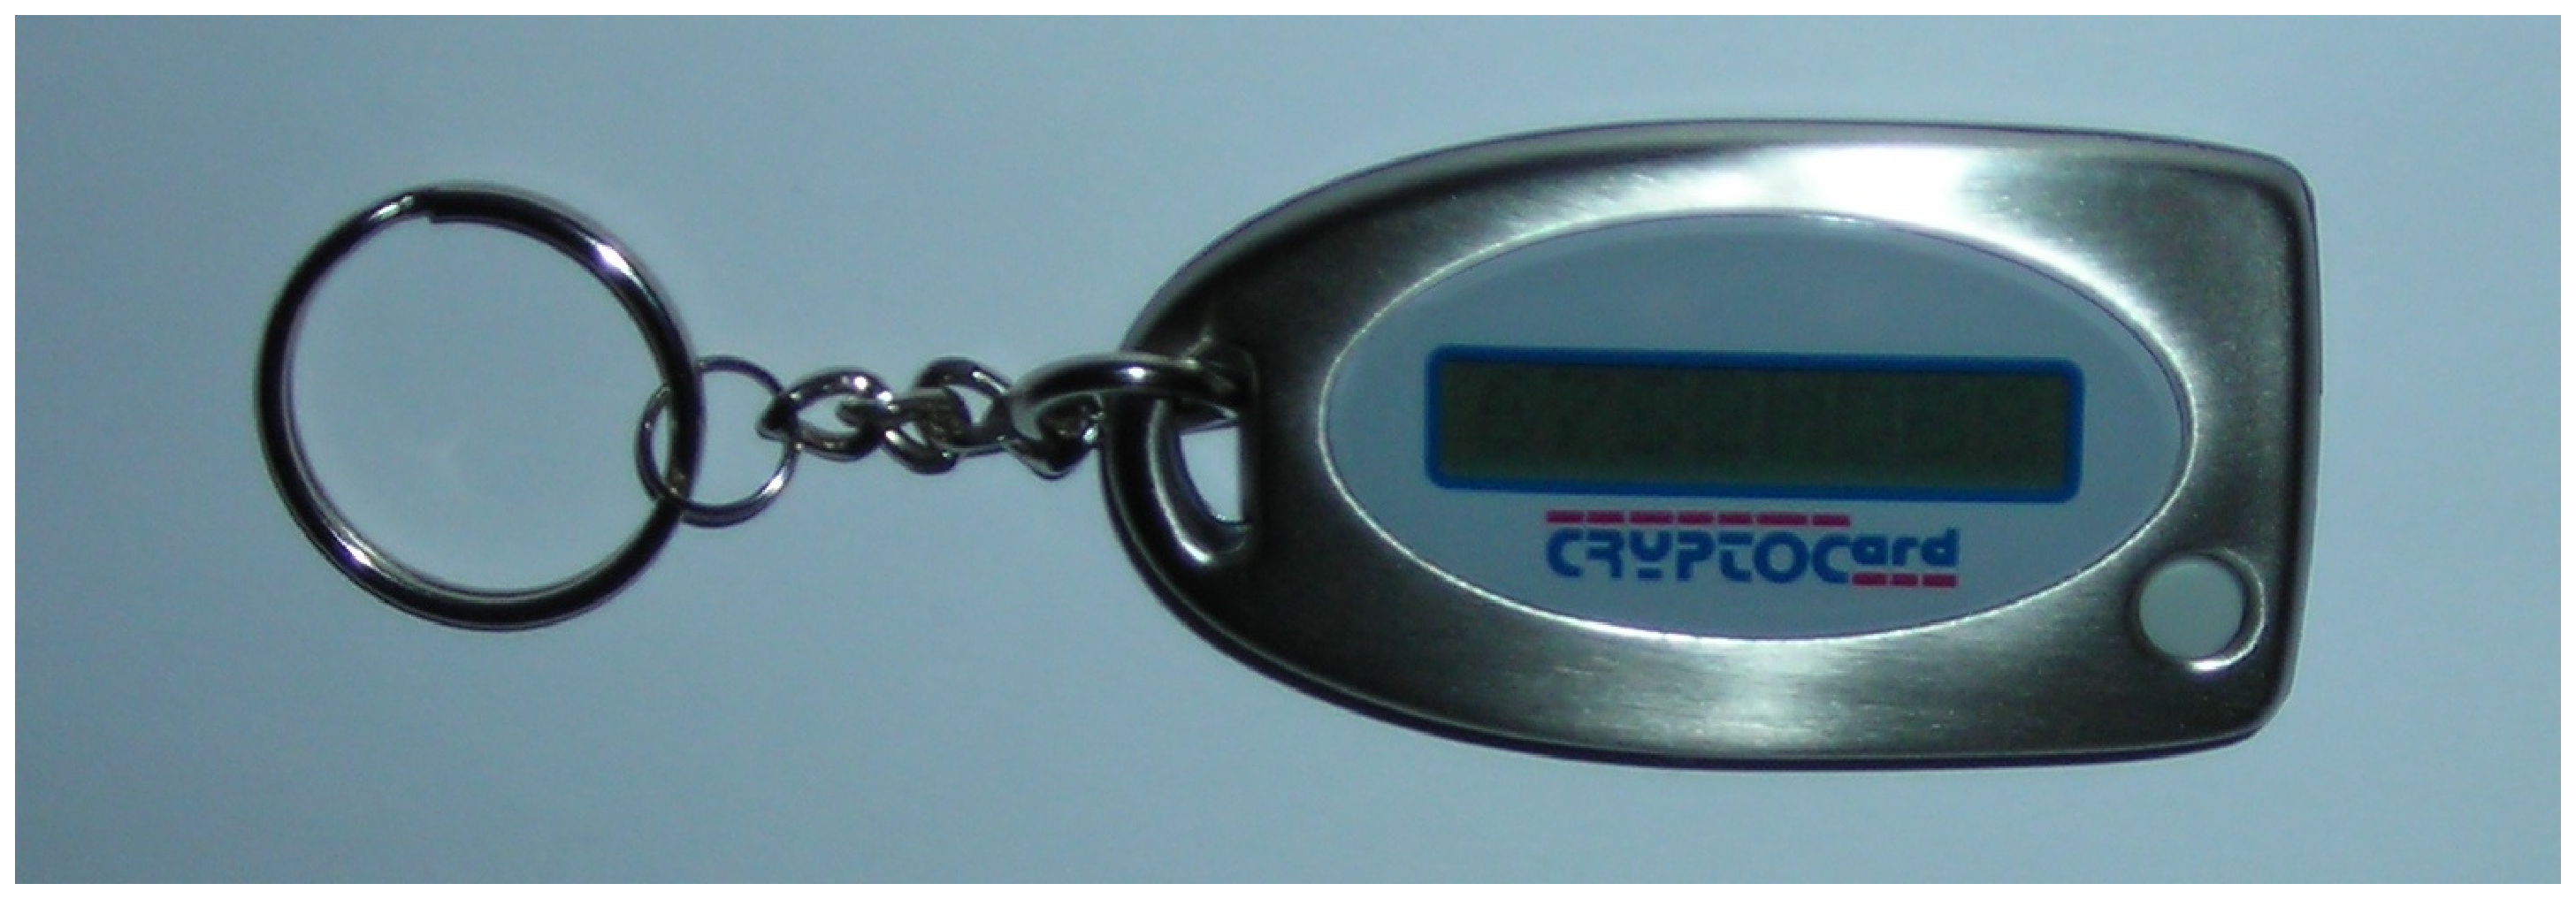
\includegraphics[width=4.6in]{c_tbg0/cckt1_01.eps}
\caption{CryptoCard KT-1 Keychain Token}
\label{fig:ctbg0:sddc0:stfa0:sovs0:00}
\end{figure}

The model of token supported by \emph{\productbasename{}}
is the CryptoCard\index{CryptoCard Corporation} 
KT-1 keychain token\index{KT-1 keychain cryptographic token} 
(Fig. \ref{fig:ctbg0:sddc0:stfa0:sovs0:00}).


On a per-user basis, logins to \emph{\productbasename{}} may be either with:

\begin{itemize}
\item Userid and password.
\item Userid, password, and OTP. 
\end{itemize}

The cryptographic basis of the CryptoCard KT-1 token and similar products
is that:

\begin{itemize}
\item The token is programmed with a key that cannot be extracted\footnote{The
      ability to extract the key from the token is equivalent to being able
      to predict all future OTPs that will be generated by the token, and hence
      would render the token useless as a security device.}, and this key is known
      to the \emph{\productbasename{}} software.
\item Mathematically, there is no way to reverse-engineer the key by observing
      OTPs generated by the token; hence there is no way to predict future
      OTPs generated by the token based on observing past OTPs.
\end{itemize}

\emph{\productbasename{}} utilizes the CryptoCard KT-1 token configured
so that each of the 8 displayed OTP characters can be one of 32 different
possibilities.\footnote{The KT-1 token can also be configured so that 
each of the 8 OTP characters can be one of 64 possibilities, leading to
$64^8 = 2.8 \times 10^{14}$ OTPs.  The base-32
OTPs were chosen because they are case-insensitive and lead to fewer user 
data entry errors.}  
The number of possible OTPs is thus $32^8 = 1.1 \times 10^{12}$.
The large number of OTPs makes a brute-force attack unattractive---even with 10 guesses
per second, the expected time to guess an OTP would be 1,700 years.

The CryptoCard KT-1 keychain token is an event-driven device---it generates
sequential OTPs according to a mathematical sequence, with one OTP generated
at each activation of the token.  The \productbasename{} software, because
it has access to the token key, is able to predict the OTPs that should be
generated by the token.  The \productbasename{} software also allows approximately
three\footnote{Configurable:  three is the default value.}
of the predicted sequential OTPs to be used, in case the KT-1 token was activated
and the OTP never used.\footnote{This might happen, for example, if the token button
is accidentally pressed by objects in the user's pockets, or if children are
allowed to play with the token.}

It can occur, however, that the KT-1 token falls out of synchronization with
the \productbasename{} software.  In this case, the token allows a resynchronization
procedure where the user enters a resynchronization string (8 digits,
allowing for $10^8$ different values).  When the token is supplied
with a resynchronization string, it resets its internal state and provides
an OTP.  This procedure allows the token and the \productbasename{} software
to be brought back into synchronization.

Note to self:  in conversation with Bill LaHam in late October 2009, Bill indicated
that the traditional approach with tokens is to have an inner window and an outer
window.  A typical inner window might be of size 3, and a typical outer window might
be of size 1000.

\begin{itemize}
\item If the token value falls within the inner window, it is authenticated without
      any other verification steps.
\item If the token value is not within the inner window but is within the outer
      window, two (additional?) consecutive values are required for authentication.
\item If the token value is not within the inner window and not within the
      outer window, some sort of resynchronization is required.
\end{itemize}

The size of the inner window is a major security risk (it raises the probability
of a successful guess), so it should be small.  The outer window is not a security
concern at all.

Need to incorporate the information from Bill into this document and the
strategy in this documennt.


%%%%%%%%%%%%%%%%%%%%%%%%%%%%%%%%%%%%%%%%%%%%%%%%%%%%%%%%%%%%%%%%%%%%%%%%%%%%%%%
%%%%%%%%%%%%%%%%%%%%%%%%%%%%%%%%%%%%%%%%%%%%%%%%%%%%%%%%%%%%%%%%%%%%%%%%%%%%%%%
%%%%%%%%%%%%%%%%%%%%%%%%%%%%%%%%%%%%%%%%%%%%%%%%%%%%%%%%%%%%%%%%%%%%%%%%%%%%%%%
\subsubsection{Additional Prudent User Authentication Practices}
%Subsubsection tag:  aap0
\label{ctbg0:sddc0:stfa0:saap0}

Even when OTPs are employed, it is not prudent to allow an attacker
a large number of authentication attempts.  The following 
prudent practices are also used by the \productbasename{} software.

\begin{enumerate}
\item Resynchronization strings are provided by the server, are generated
      as sequential values (``00000000'', ``00000001'', ``00000002'', etc.),
      and are only reused with a period of $10^8$.  (This is designed to
      elmiminate an attacker's ability to observe how a token responds to
      a specific resynchronization string and to reuse this information as
      part of an attack.)
\item Unsuccessful authentication attempts that involve an invalid userid
      are logged but otherwise simply ignored.
\item Unsuccessful authentication attempts that involve a valid userid but 
      both invalid password and invalid OTP are logged but otherwise
      simply ignored.
\item Unsuccessful authentication attempts involving a valid userid and
      either a valid password and invalid OTP or invalid password and valid
      OTP\footnote{In the case of a user for whom two-factor authentication
      is not enabled, valid userid and invalid password are treated as described
      here---the key element is that the attacker appears to be ``one piece''
      away from a successful attack.} 
      are treated more aggressively because this case hints at an attacker
      who has obtained a user's password but has no token or has obtained a token
      but does not have the user's password, and is ``fishing'' for the missing
      piece.  If a sufficient number of these attacks directed at the userid have
      occurred from the same IP in a short period of time, login ability for
      this userid from the affected IP is silently disabled for a period of 
      time.\footnote{\emph{Silently} means that the web interface will only indicate
      unsuccessful authentication, and will give no indication that a probable attack
      has been detected or that authentication for the affected userid from the 
      affected IP is temporarily impossible.  \emph{Disabled} means that even if
      correct authentication credentials are provided, they will be rejected.  The
      purpose of this policy is to eliminate the ability of an attacker to try large
      numbers of attacks in a short period of time, and to deny an attacker information
      about how to better mount an attack.} 
\end{enumerate}


%%%%%%%%%%%%%%%%%%%%%%%%%%%%%%%%%%%%%%%%%%%%%%%%%%%%%%%%%%%%%%%%%%%%%%%%%%%%%%%
%%%%%%%%%%%%%%%%%%%%%%%%%%%%%%%%%%%%%%%%%%%%%%%%%%%%%%%%%%%%%%%%%%%%%%%%%%%%%%%
%%%%%%%%%%%%%%%%%%%%%%%%%%%%%%%%%%%%%%%%%%%%%%%%%%%%%%%%%%%%%%%%%%%%%%%%%%%%%%%
\subsection{Per-User Authentication and Administrative Rights}
%Subsection tag:  pua0
\label{ctbg0:sddc0:spua0}

\emph{\productbasename{}-\productversion{}} has no notion of an
``administrative'' or ``master'' password.  Each individual user
logs in using a user-ID identifying themselves, even to perform
administrative tasks.

Tasks are divided into two groups:

\begin{itemize}
\item Ordinary tasks (that typically view data or moves workproducts
      through a process).
\item Administrative tasks that:
      \begin{itemize}
      \item Represent administration of the \emph{\productbasename{}-\productversion{}}
            software, rather than usage of the software; AND/OR
      \item Are sensitive to mistakes, and could destroy or corrupt 
            data.
      \end{itemize}
\end{itemize}

\emph{\productbasename{}-\productversion{}} allows two types of logins:

\begin{itemize}
\item \emph{Normal login}:  the user has priveleges only to perform
      non-administrative tasks.
\item \emph{Administrative login}:  the user has priveleges to perform
      non-administrative and administrative tasks.
\end{itemize}

In order to perform a normal login, the user simply enters their
user-ID (``\emph{jsmith}'', for example) as the user-ID when logging in.

In order to perform an administrative login, the user enters their
user-ID postfixed with an asterisk (``\emph{jsmith*}'', for
example as the user-ID when logging in.  When a user has performed an
administrative login, the color scheme used for the web pages
is based on the color red rather than on blues and grays.

The only way to switch between normal and administrative logins 
is by logging out and logging in again.


%%%%%%%%%%%%%%%%%%%%%%%%%%%%%%%%%%%%%%%%%%%%%%%%%%%%%%%%%%%%%%%%%%%%%%%%%%%%%%%
%%%%%%%%%%%%%%%%%%%%%%%%%%%%%%%%%%%%%%%%%%%%%%%%%%%%%%%%%%%%%%%%%%%%%%%%%%%%%%%
%%%%%%%%%%%%%%%%%%%%%%%%%%%%%%%%%%%%%%%%%%%%%%%%%%%%%%%%%%%%%%%%%%%%%%%%%%%%%%%
\subsection{\emph{su} Logins}
%Subsection tag:  sul0
\label{ctbg0:sddc0:ssul0}

\index{su login@\emph{su} login}It is helpful in some
situations to be able to log in as a different user.  Such logins are 
called \emph{su} logins (after the *nix \emph{su} command).  These situations
include:

\begin{itemize}
\item Testing.
\item Performing actions on behalf of other users.
\end{itemize}

In order to \emph{su} as another user, the user logging in
must enter a user-ID of the form ``\emph{actualuser as suuser}''
as the user-ID when logging in.  ``\emph{actualuser as suuser*}'' can
also be used for an \emph{su} administrative login.

In order to perform an \emph{su} login as another user, a user
must have strictly superior priveleges.  Specifically:

\begin{itemize}
\item The \emph{seclvl} of the actual user must be 
      a smaller integer than the \emph{seclvl} of the \emph{su} user.
\item The actual user must have at least every permission attribute
      that the \emph{su} user has.
\item For those permission attributes that are ranked, the ranking
      must be at least as great as the \emph{su} user.
\end{itemize}

Once the login is complete, the \emph{su} login is indistinguishable from an
actual login except for the log entries.  The session maintained does
not contain any state to indicate that it represents an \emph{su} login.


%%%%%%%%%%%%%%%%%%%%%%%%%%%%%%%%%%%%%%%%%%%%%%%%%%%%%%%%%%%%%%%%%%%%%%%%%%%%%%%
%%%%%%%%%%%%%%%%%%%%%%%%%%%%%%%%%%%%%%%%%%%%%%%%%%%%%%%%%%%%%%%%%%%%%%%%%%%%%%%
%%%%%%%%%%%%%%%%%%%%%%%%%%%%%%%%%%%%%%%%%%%%%%%%%%%%%%%%%%%%%%%%%%%%%%%%%%%%%%%
\subsection{Multiple Logins}
%Subsection tag:  mlo0
\label{ctbg0:sddc0:smlo0}

The maximum number of logins per user is a global configuration
constant, defined in the \texttt{config.inc} \emph{PHP} file.
The default value is 3.

If the maximum number of logins is reached and another user 
successfully authenticates with the
same user-ID, the session with the oldest creation time is destroyed (forcibly
logging out this instance of the user).


%%%%%%%%%%%%%%%%%%%%%%%%%%%%%%%%%%%%%%%%%%%%%%%%%%%%%%%%%%%%%%%%%%%%%%%%%%%%%%%
%%%%%%%%%%%%%%%%%%%%%%%%%%%%%%%%%%%%%%%%%%%%%%%%%%%%%%%%%%%%%%%%%%%%%%%%%%%%%%%
%%%%%%%%%%%%%%%%%%%%%%%%%%%%%%%%%%%%%%%%%%%%%%%%%%%%%%%%%%%%%%%%%%%%%%%%%%%%%%%
\subsection{The Standard Hash Function}
%Subection tag:  shf0
\label{ctbg0:sddc0:sshf0}

The \index{standard hash function}\emph{standard hash function} is the
standard way that the \emph{\productbasename{}-\productversion{}} software
maps between a number of arbitrary input arguments and a 160-bit
SHA1 hash.  The standard hash function involves mixing
the input arguments with a secret hash key
(described in \S{}\ref{ctbg0:sdty0:sthk0}).

If `+' is used to represent the string concatenation operation, all
arguments $a_i$ that are not strings are converted to string format, then the
SHA1 hash is applied to the concatenation of the secret hash key $k_h$ and the
arguments $a_i$ as described by the first few patterns below.

\begin{eqnarray}
\nonumber
SHF_1(a_1)              & = & SHA1(k_h + a_1 + k_h) \\
\label{eq:ctbg0:sddc0:sshf0:01}
SHF_2(a_1, a_2)         & = & SHA1(k_h + a_1 + k_h + a_2 + k_h) \\
\nonumber
SHF_3(a_1, a_2, a_3)    & = & SHA1(k_h + a_1 + k_h + a_2 + k_h + a_3 + k_h)
\end{eqnarray}

Note that the hash functions above are designed so that it should be
impossible for an attacker to predict the hash that will be generated
for a given set of input arguments $a_i$ unless the hash key $k_h$ has
been compromised.


%%%%%%%%%%%%%%%%%%%%%%%%%%%%%%%%%%%%%%%%%%%%%%%%%%%%%%%%%%%%%%%%%%%%%%%%%%%%%%%
%%%%%%%%%%%%%%%%%%%%%%%%%%%%%%%%%%%%%%%%%%%%%%%%%%%%%%%%%%%%%%%%%%%%%%%%%%%%%%%
%%%%%%%%%%%%%%%%%%%%%%%%%%%%%%%%%%%%%%%%%%%%%%%%%%%%%%%%%%%%%%%%%%%%%%%%%%%%%%%
\subsection{Storage of User Passwords}
%Subection tag:  sup0
\label{ctbg0:sddc0:ssup0}

It is generally known that individuals tend to choose identical or similar
passwords across many different computing applications.  For that reason, it
is important to safeguard the passwords used with
\emph{\productbasename{}-\productversion{}}.  Although 
\emph{\productbasename{}-\productversion{}} may be a relatively unimportant
product to a user, the other software products with which the user is
unwisely using the same password may be important.
It is important to protect passwords.

Passwords are never stored in \emph{\productbasename{}-\productversion{}}.
Instead, the $SHF1(\cdot{})$ of the password (as described in
Eq. \ref{eq:ctbg0:sddc0:sshf0:01}) is stored.

It is possible, although extremely unlikely, that two non-identical 
passwords would have the same stored hash.  Assuming that 
a typical user is comfortable using 62 characters (26 lower-case letters, 26 upper-case
letters, and 10 digits) as part of a password, an approximation of how many
password characters $n$ a 160-bit hash is equivalent to can be obtained by
solving:

\begin{equation}
62^n = 2^{160}
\end{equation}

\begin{equation}
n = \frac{160 \log 2}{\log 62} \approx 27
\end{equation}

\noindent{}Thus, a hash collision involving two different typical passwords is
\emph{very} unlikely.

If the stored password hash is compromised but the hash key is not, no attack
is possible except brute-force password guessing (with no advantage gained
due to compromise of the stored password hash).

If both the stored password hash and the hash key are compromised, the best
attack possible is a dictionary attack.  This may or may not be fruitful,
depending on the strength of password chosen by the user.


%%%%%%%%%%%%%%%%%%%%%%%%%%%%%%%%%%%%%%%%%%%%%%%%%%%%%%%%%%%%%%%%%%%%%%%%%%%%%%%
%%%%%%%%%%%%%%%%%%%%%%%%%%%%%%%%%%%%%%%%%%%%%%%%%%%%%%%%%%%%%%%%%%%%%%%%%%%%%%%
%%%%%%%%%%%%%%%%%%%%%%%%%%%%%%%%%%%%%%%%%%%%%%%%%%%%%%%%%%%%%%%%%%%%%%%%%%%%%%%
\subsection{Internal Representation of Time}
%Subection tag:  rti0
\label{ctbg0:sddc0:srti0}

It is very common for a project to involve individuals from several
countries.  In this context, it is important to have no ambiguity
about the values of time recorded in a database.

The following design decisions have been made:

\begin{itemize}
\item All stored time values corresponding to events will
      be in \index{UTC}UTC.
\item In many contexts, the stored time values will also
      be presented in local time.  (However, 
      presentation in local time alone is strongly discouraged---UTC should be the norm
      for collaboration.)
\item The calendaring range for date functionality will be
      from 1900 through 2999.\footnote{This represents a
      span of approximately 34,713,000,000 seconds.  Although this
      exceeds the range of a 32-bit representation, it comfortably
      fits in a 64-bit representation.}
\end{itemize}

%%%%%%%%%%%%%%%%%%%%%%%%%%%%%%%%%%%%%%%%%%%%%%%%%%%%%%%%%%%%%%%%%%%%%%%%%%%%%%%
%%%%%%%%%%%%%%%%%%%%%%%%%%%%%%%%%%%%%%%%%%%%%%%%%%%%%%%%%%%%%%%%%%%%%%%%%%%%%%%
%%%%%%%%%%%%%%%%%%%%%%%%%%%%%%%%%%%%%%%%%%%%%%%%%%%%%%%%%%%%%%%%%%%%%%%%%%%%%%%
\section{\emph{PHP} Design Decisions and Discussion}
%Section tag:  php0
\label{ctbg0:sphp0}


%%%%%%%%%%%%%%%%%%%%%%%%%%%%%%%%%%%%%%%%%%%%%%%%%%%%%%%%%%%%%%%%%%%%%%%%%%%%%%%
%%%%%%%%%%%%%%%%%%%%%%%%%%%%%%%%%%%%%%%%%%%%%%%%%%%%%%%%%%%%%%%%%%%%%%%%%%%%%%%
%%%%%%%%%%%%%%%%%%%%%%%%%%%%%%%%%%%%%%%%%%%%%%%%%%%%%%%%%%%%%%%%%%%%%%%%%%%%%%%
\subsection{Native Integer Size}
%Subsection tag:  nis0
\label{ctbg0:sphp0:snis0}

Prior to \emph{PHP} 5, \emph{PHP} integers were the same size as the native
integer of the underlying machine.  With some machines this is 32 bits, and with
other machines this is 64 bits.

In the case of a 32-bit integer, the range of values that can be represented
by an integer $x$ is

\begin{eqnarray}
-(2^{31})      & \leq \; x \; \leq & 2^{31} - 1\\
\nonumber -2,147,483,648 & \leq \; x \; \leq & 2,147,483,647 .
\end{eqnarray}

It is necessary to ensure that 64-bit integer arithmetic is available from 
\emph{PHP} for the following reasons:

\begin{itemize}
\item Certain of the database tables may exceed $2^{31}-1$ records or,
      due to addition and deletion of records, have key values that
      exceed $2^{31}-1$.
\item The number of seconds since the Unix epoch will exceed $2^{31}-1$ seconds
      in 2037 A.D\@.  \emph{\productbasename{}} must be able to perform
      date calculations further into the future than 2037 A.D., and so
      integers exceeding 32 bits in size would be convenient. 
\end{itemize}

To work around the limitations of 32-bit integers, the following strategy
is used:

\begin{itemize}
\item Integers that may exceed 32 bits are represented as strings rather than
      as integers, and \emph{PHP}'s \emph{bcmath} library is used to manipulate
      these strings.
\item In issuing \emph{MySQL} statements that specify integers larger than 32 bits,
      no special action is required, as an SQL statement is ultimately only a string.
      However, when obtaining result sets from \emph{MySQL} that may involve
      integers larger than 32 bits, special SQL statements that cast the portions of
      the result set to a string are used.
\end{itemize}

The strategy described above will work equally well with \emph{PHP} when 
64-bit integers are directly supported, but with slight inefficiency.


%%%%%%%%%%%%%%%%%%%%%%%%%%%%%%%%%%%%%%%%%%%%%%%%%%%%%%%%%%%%%%%%%%%%%%%%%%%%%%%
%%%%%%%%%%%%%%%%%%%%%%%%%%%%%%%%%%%%%%%%%%%%%%%%%%%%%%%%%%%%%%%%%%%%%%%%%%%%%%%
%%%%%%%%%%%%%%%%%%%%%%%%%%%%%%%%%%%%%%%%%%%%%%%%%%%%%%%%%%%%%%%%%%%%%%%%%%%%%%%
\section{Web Interface Design Decisions and Discussion}
%Section tag:  wid0
\label{ctbg0:swid0}


%%%%%%%%%%%%%%%%%%%%%%%%%%%%%%%%%%%%%%%%%%%%%%%%%%%%%%%%%%%%%%%%%%%%%%%%%%%%%%%
%%%%%%%%%%%%%%%%%%%%%%%%%%%%%%%%%%%%%%%%%%%%%%%%%%%%%%%%%%%%%%%%%%%%%%%%%%%%%%%
%%%%%%%%%%%%%%%%%%%%%%%%%%%%%%%%%%%%%%%%%%%%%%%%%%%%%%%%%%%%%%%%%%%%%%%%%%%%%%%
\subsection{Client IP Address Modified During Session}
%Subsection tag:  ipa0
\label{ctbg0:swid0:sipa0}

Newsgroup posters have identified that an IP address may shift during a
session (due to DHCP lease lifetimes and so on).  For this reason, an
IP address that shifts during a session will result in a warning in the
logs rather than termination of the session.\footnote{Termination of the
session is a forced immediate logout.}


%%%%%%%%%%%%%%%%%%%%%%%%%%%%%%%%%%%%%%%%%%%%%%%%%%%%%%%%%%%%%%%%%%%%%%%%%%%%%%%
%%%%%%%%%%%%%%%%%%%%%%%%%%%%%%%%%%%%%%%%%%%%%%%%%%%%%%%%%%%%%%%%%%%%%%%%%%%%%%%
%%%%%%%%%%%%%%%%%%%%%%%%%%%%%%%%%%%%%%%%%%%%%%%%%%%%%%%%%%%%%%%%%%%%%%%%%%%%%%%
\section{\emph{PHP}-Spawned Program Design Decisions and Discussion}
%Section tag:  phs0
\label{ctbg0:sphs0}


%%%%%%%%%%%%%%%%%%%%%%%%%%%%%%%%%%%%%%%%%%%%%%%%%%%%%%%%%%%%%%%%%%%%%%%%%%%%%%%
%%%%%%%%%%%%%%%%%%%%%%%%%%%%%%%%%%%%%%%%%%%%%%%%%%%%%%%%%%%%%%%%%%%%%%%%%%%%%%%
%%%%%%%%%%%%%%%%%%%%%%%%%%%%%%%%%%%%%%%%%%%%%%%%%%%%%%%%%%%%%%%%%%%%%%%%%%%%%%%
\section{\emph{cron}-Job Design Decisions and Discussion}
%Section tag:  cjd0
\label{ctbg0:scjd0}


%%%%%%%%%%%%%%%%%%%%%%%%%%%%%%%%%%%%%%%%%%%%%%%%%%%%%%%%%%%%%%%%%%%%%%%%%%
\noindent\begin{figure}[!b]
\noindent\rule[-0.25in]{\textwidth}{1pt}
\begin{tiny}
\begin{verbatim}
$RCSfile: c_tbg0.tex,v $
$Source: /home/dashley/cvsrep/e3ft_gpl01/e3ft_gpl01/webprojs/pamc/gen_a/docs/manual/man_a/c_tbg0/c_tbg0.tex,v $
$Revision: 1.35 $
$Author: dashley $
$Date: 2009/11/01 02:42:55 $
\end{verbatim}
\end{tiny}
\noindent\rule[0.25in]{\textwidth}{1pt}
\end{figure}

%%%%%%%%%%%%%%%%%%%%%%%%%%%%%%%%%%%%%%%%%%%%%%%%%%%%%%%%%%%%%%%%%%%%%%%%%%%%%%%
%$Log: c_tbg0.tex,v $
%Revision 1.35  2009/11/01 02:42:55  dashley
%Edits.
%
%Revision 1.34  2007/07/13 02:38:04  dashley
%Edits.
%
%Revision 1.33  2007/07/13 01:19:57  dashley
%Edits.
%
%Revision 1.32  2007/07/11 14:31:40  dashley
%Edits.
%
%Revision 1.31  2007/07/07 23:12:54  dashley
%Edits.
%
%Revision 1.30  2007/07/07 03:49:58  dashley
%Edits.
%
%Revision 1.29  2007/07/07 03:31:53  dashley
%Edits.
%
%Revision 1.28  2007/07/04 22:41:27  dashley
%Edits.
%
%Revision 1.27  2007/07/04 05:09:24  dashley
%Edits.
%
%Revision 1.26  2007/07/02 01:32:50  dashley
%Edits.
%
%Revision 1.25  2007/07/01 03:07:14  dashley
%Edits.
%
%Revision 1.24  2007/06/24 20:21:55  dashley
%Edits.
%
%Revision 1.23  2007/06/24 16:35:48  dashley
%Edits.
%
%Revision 1.22  2007/06/24 02:16:50  dashley
%Edits.
%
%Revision 1.21  2007/06/24 00:42:20  dashley
%Edits.
%
%Revision 1.20  2007/06/23 22:16:10  dashley
%Safety checkin before graphics file renaming.
%
%Revision 1.19  2007/06/21 03:26:10  dashley
%Edits.
%
%Revision 1.18  2007/06/21 03:21:32  dashley
%Edits.
%
%Revision 1.17  2007/06/21 03:09:39  dashley
%Edits.
%
%Revision 1.16  2007/06/14 01:59:36  dashley
%Edits.
%
%Revision 1.15  2007/06/10 18:03:20  dashley
%Edits.
%
%Revision 1.14  2007/06/10 16:04:12  dashley
%Edits.
%
%Revision 1.13  2007/06/10 05:01:40  dashley
%Edits.
%
%Revision 1.12  2007/06/10 03:42:30  dashley
%Edits.
%
%Revision 1.11  2007/06/10 02:30:17  dashley
%Initial checkin.phpstatic01.dsf
%
%Revision 1.10  2007/06/07 20:05:20  dashley
%Edits.
%
%Revision 1.9  2007/06/07 05:03:20  dashley
%Edits.
%
%Revision 1.8  2007/06/06 01:55:08  dashley
%Multiply-defined label corrected.
%
%Revision 1.7  2007/06/06 00:32:07  dashley
%Edits.
%
%Revision 1.6  2007/06/05 15:47:12  dashley
%Structural edits.
%
%Revision 1.5  2007/06/05 00:39:55  dashley
%Edits.
%
%Revision 1.4  2007/06/04 03:26:55  dashley
%Edits.
%
%Revision 1.3  2007/06/03 23:15:27  dashley
%Edits.
%
%Revision 1.2  2007/06/03 07:57:10  dashley
%Edits.
%
%Revision 1.1  2007/06/03 07:16:08  dashley
%Initial checkin.
%
%End of $RCSfile: c_tbg0.tex,v $.
